\chapter{Sentence similarity and embeddings}
% TODO include all equations/tables/pictures in latex figures only! Examples are given below.
\section{\label{sec:level1} Introduction}
% TODO:  summarize the topic, without equations/figures and without using abbreviations (semi-supervised learning and NOT SSL). Should be around 300 words (+/- 50 words). 

Sentence similarity and embeddings are an extension of character-level and word-level embeddings that are common building blocks of downstream natural language processing tasks. Embeddings address the problem of sparsity in one-hot encoding by using surrogate neural networks to create dense representations of text that model semantic similarity. Initial approaches to embeddings, such as word2vec and gloVe, have been sufficient for tasks that do not require explicitly comparing phrases, sentences, or documents. Tasks that require this multi-word information, such as information retrieval or document classification, have struggled to incorporate word level embeddings. Many approaches applied reweighting or normalization methods to word level embeddings to infer the embedding for a sentence. However, this does not preserve word order and falsely assumes that the meaning of a phrase or sentence is nothing more than the superficial combination of the meaning of individual words. 

A number of different approaches to sentence embeddings have been proposed to address the limitations of extracting multi-word information from word embeddings. These approaches introduce novel ways to deal with polysemy, out of vocabulary words, word order preservation, sensitivity to sentence form, and transfer learning. This chapter will discuss four such methods, namely doc2vec, skip-thoughts, quick-thoughts, and the universal sentence encoder. 


\section{\label{keywords} Keywords}
% TODO: write a comma-separated list of keywords for your topic. The order of the keywords should be the order in which you think a student who wants to learn your topic should study these keywords in order to learn the topic. The last keyword in the list should be the name of your topic. An example is shown below:
word embeddings, character embeddings, word2vec, gloVe, CBOW, skip-gram, doc2vec, gated recurrent units, recurrent neural networks, long-short term memory networks, skip-thoughts, quick-thoughts, deep averaging network, attention, transformers, transfer learning, universal sentence embedding, sentence embeddings

\section{\label{sec:level3} Background material}
% TODO: describe math and any background material not covered in the introduction which you think is useful for understanding the papers

\subsection{word2vec}

This is a citation for word2vec \cite{word2vec}

\subsection{gloVe}

This is a citation for glove \cite{glove}

\subsection{Gated recurrent units}

Citation for gated recurrent units \cite{gru}

\subsection{Deep averaging network}

Citation for DAN \cite{dan}

\subsection{Self attention}

Citation for attention \cite{attention}

\section{\label{sec:level4} Presentation of papers}
\subsection{Summary of Distributed Representations of Sentences and Documents}
% TODO: Summarize the motivation, goals, techniques and results of the paper. Fill {Paper 1} with the exact title of the paper as found in your .bib file. 
Doc2vec citation \cite{conf/icml/LeM14}.
\begin{figure}
\centering
$$H^{(l+1)} = \sigma (\widetilde{D}^{\frac{-1}{2}}\widetilde{A}\widetilde{D}^{\frac{-1}{2}}H^{(l)}W^{(l)}),$$ where $\widetilde{A} = A + I_N$, $\widetilde{D}_{ii} = \sum_{j}\widetilde{A}_{ij}$, $W^{(l)}$, $H^{(l)} \in R^{NxD}$ and $H^{(0)} = X$. 
\caption{These equations describe the layer-wise propagation rule for the multi-layer Graph Convolutional Network.}
\label{fig:gcn}
\end{figure}

\begin{figure}
\centering
  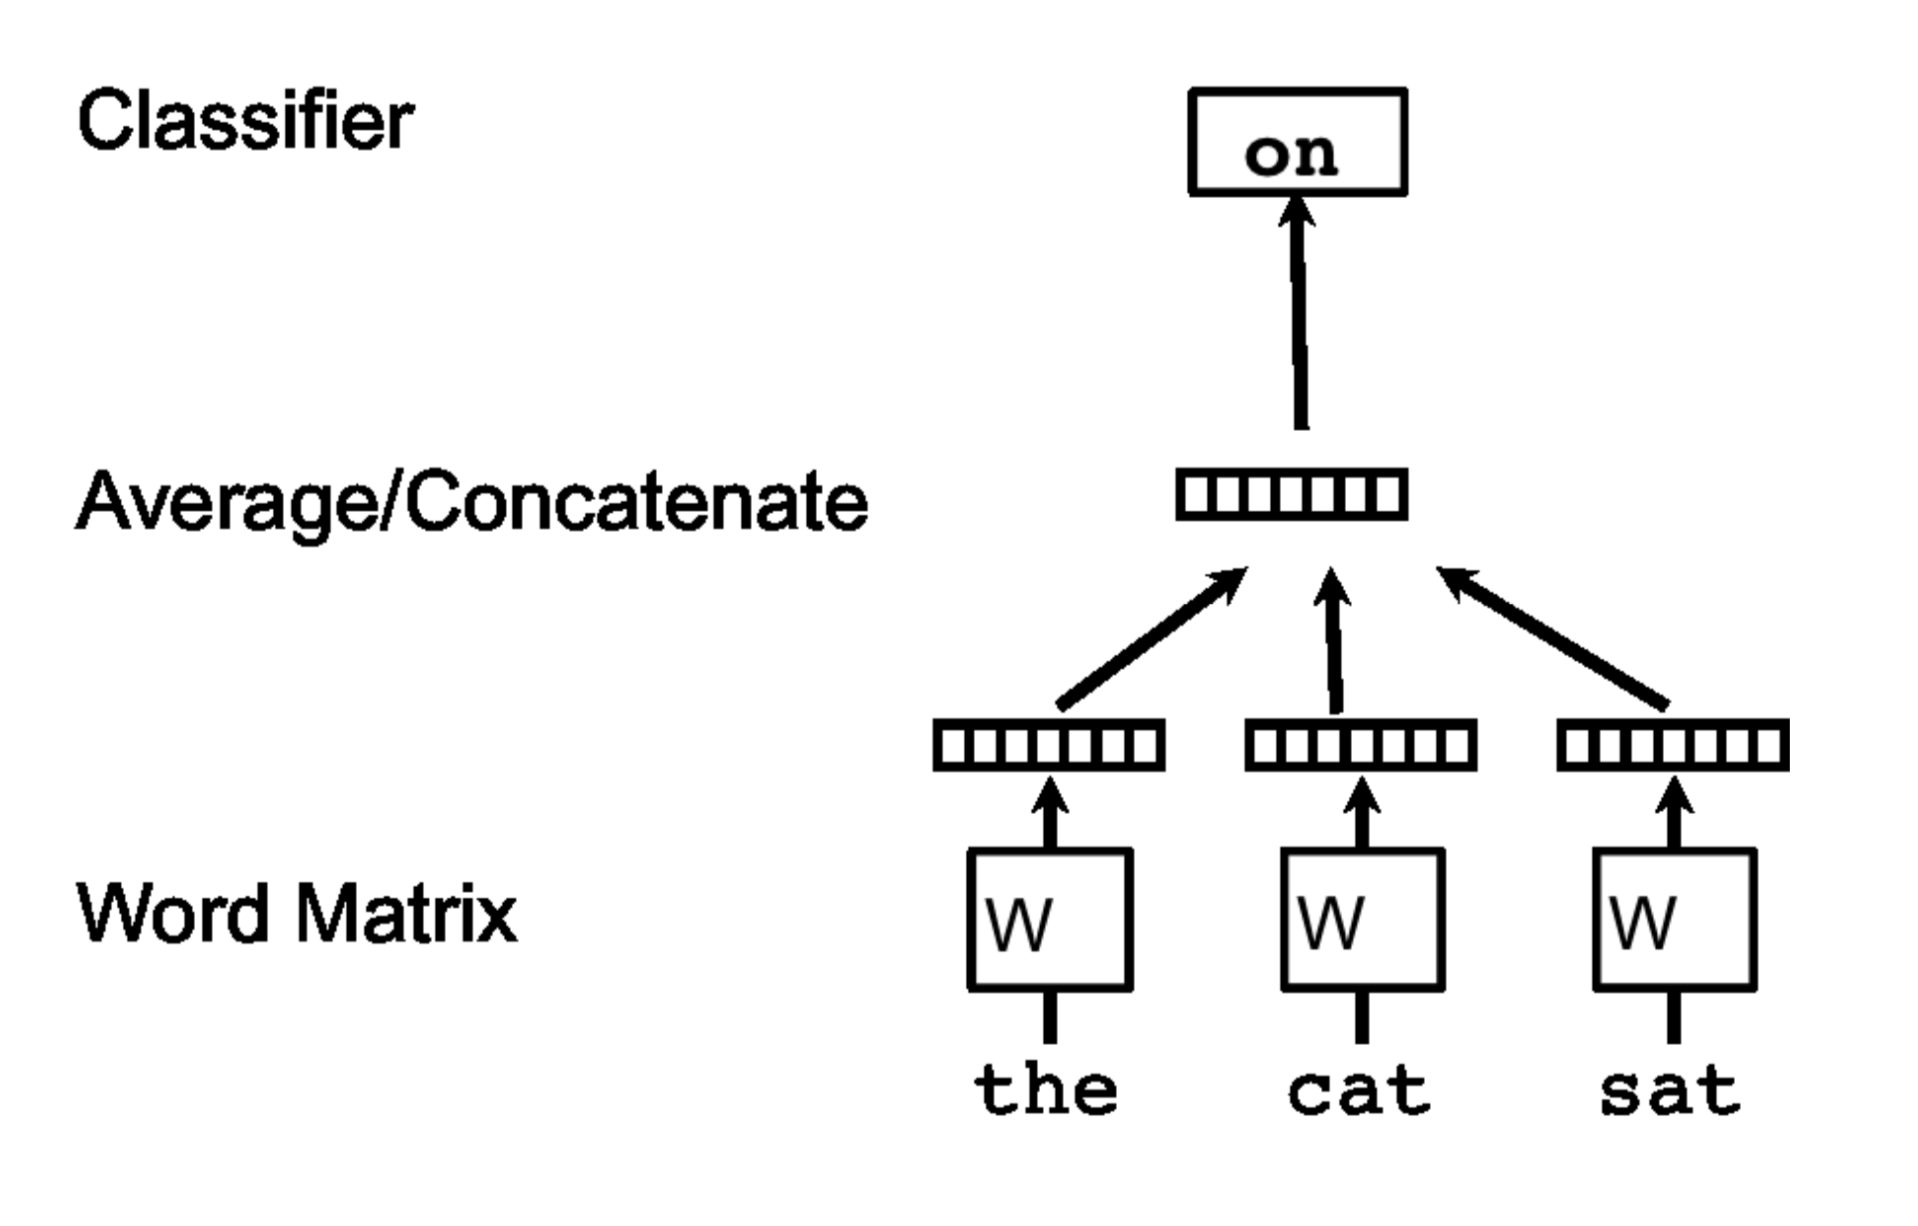
\includegraphics[width=.5\linewidth]{files/doc2vec-1.png}
  \caption{A variational autoencoder models the latent variable z from which the data x is generated.}
  \label{fig:vae}
\end{figure}

\begin{figure}
\centering
  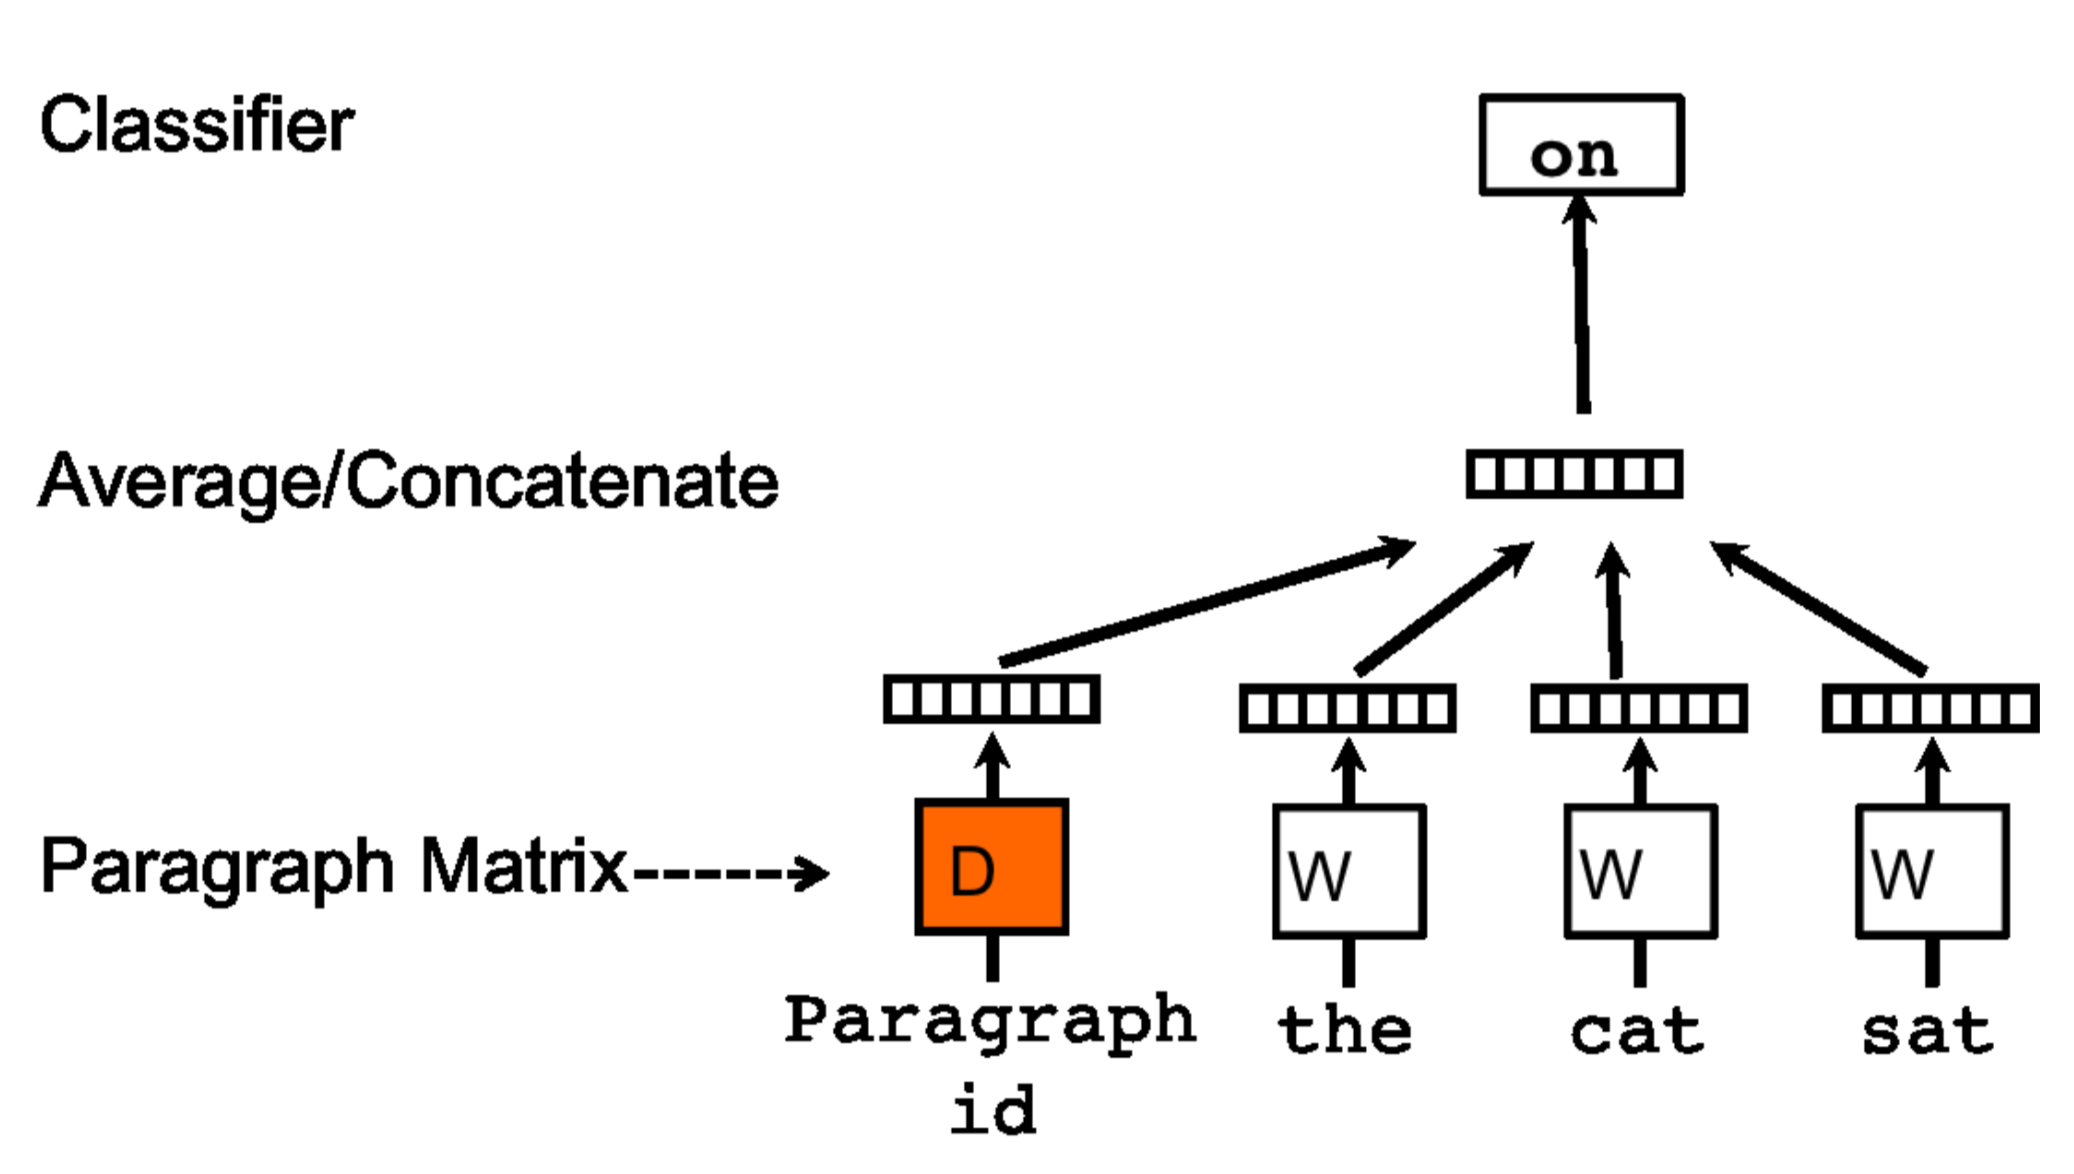
\includegraphics[width=.5\linewidth]{files/doc2vec-2.png}
  \caption{A variational autoencoder models the latent variable z from which the data x is generated.}
  \label{fig:vae}
\end{figure}

\begin{figure}
\centering
  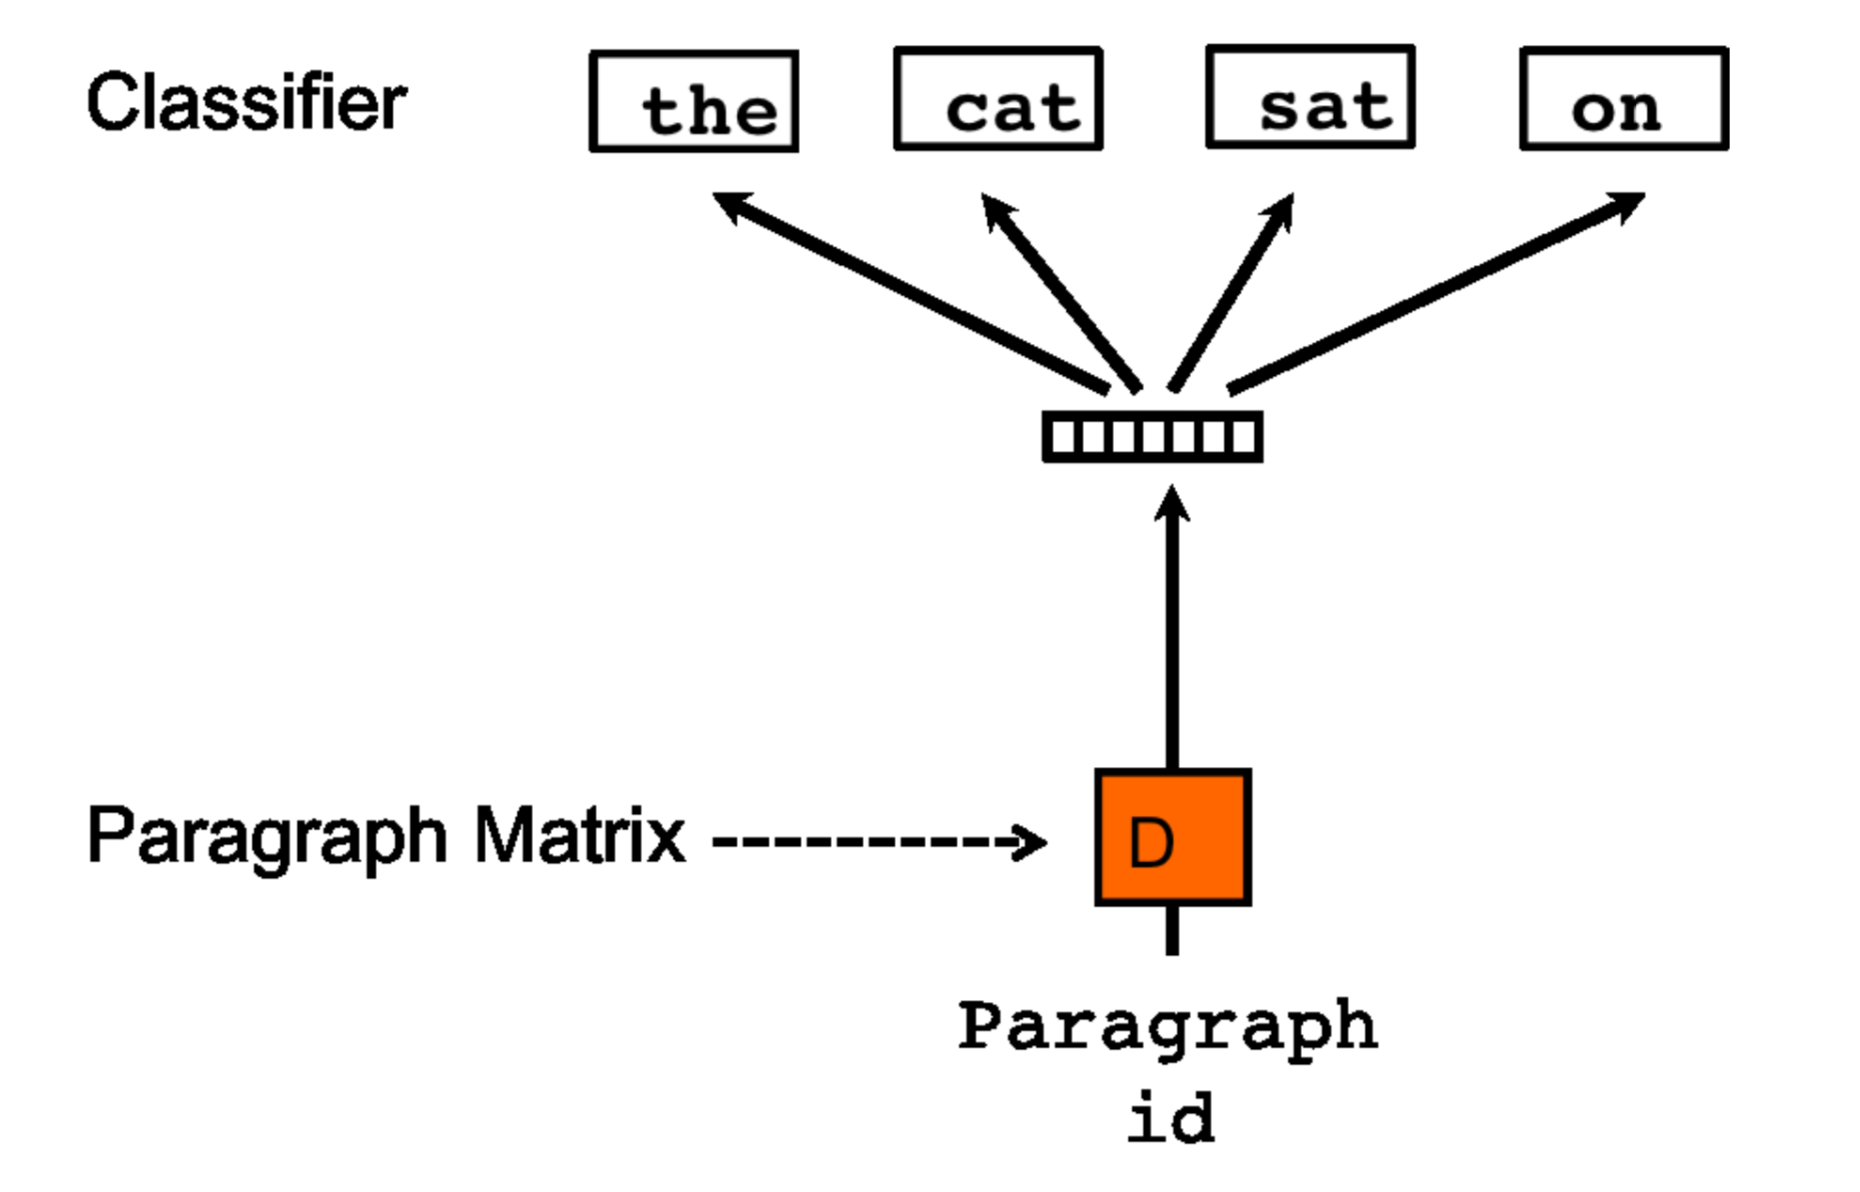
\includegraphics[width=.5\linewidth]{files/doc2vec-3.png}
  \caption{A variational autoencoder models the latent variable z from which the data x is generated.}
  \label{fig:vae}
\end{figure}

\begin{figure}
\centering
  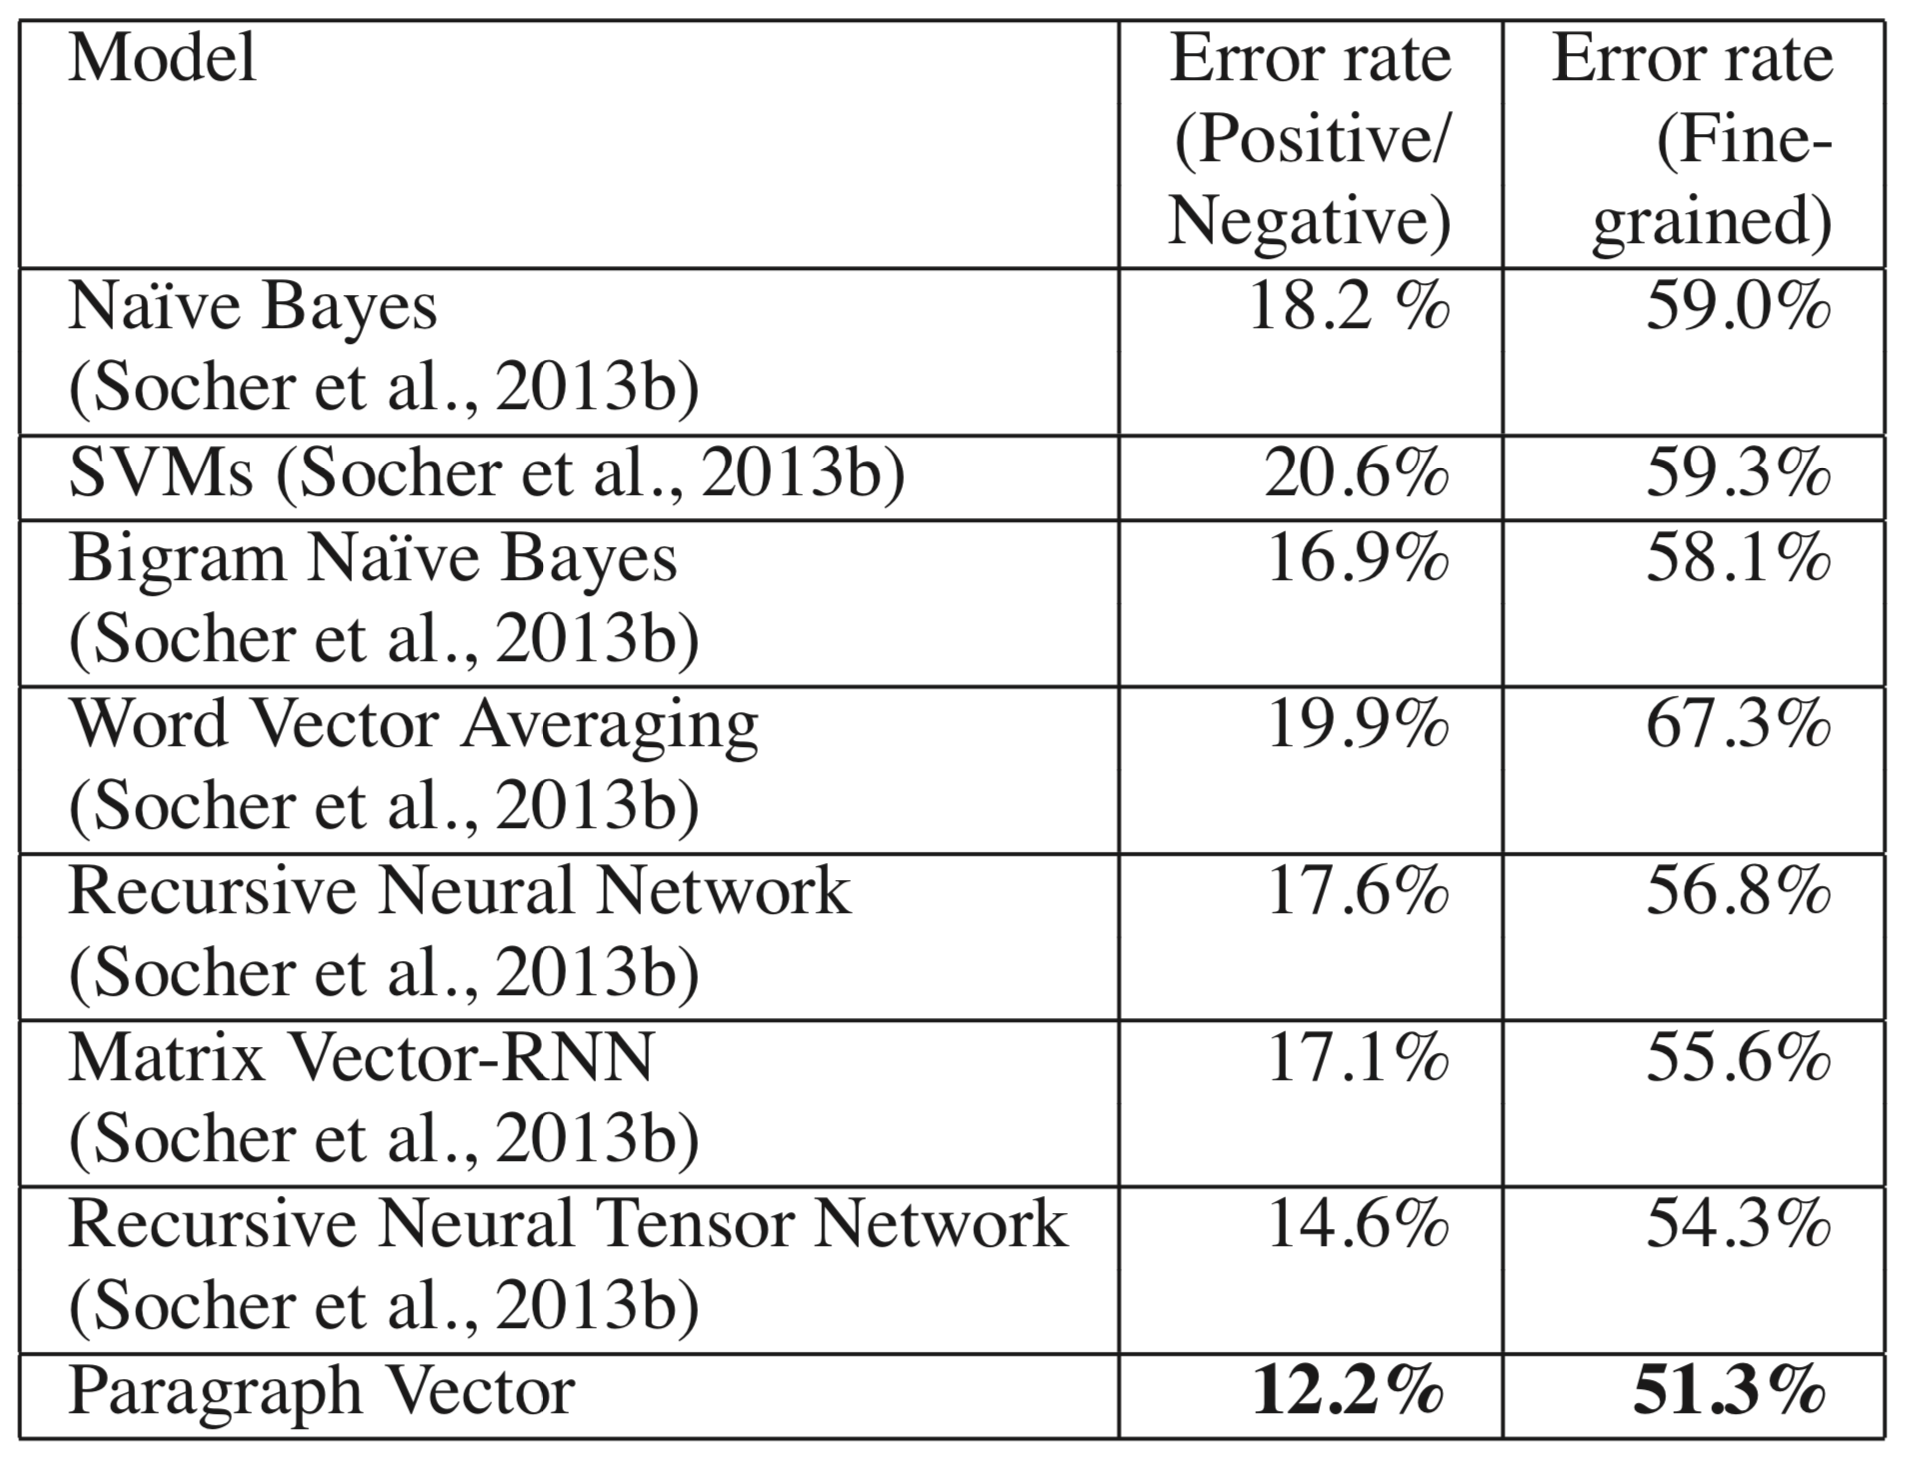
\includegraphics[width=.5\linewidth]{files/doc2vec-4.png}
  \caption{A variational autoencoder models the latent variable z from which the data x is generated.}
  \label{fig:vae}
\end{figure}

\begin{figure}
\centering
  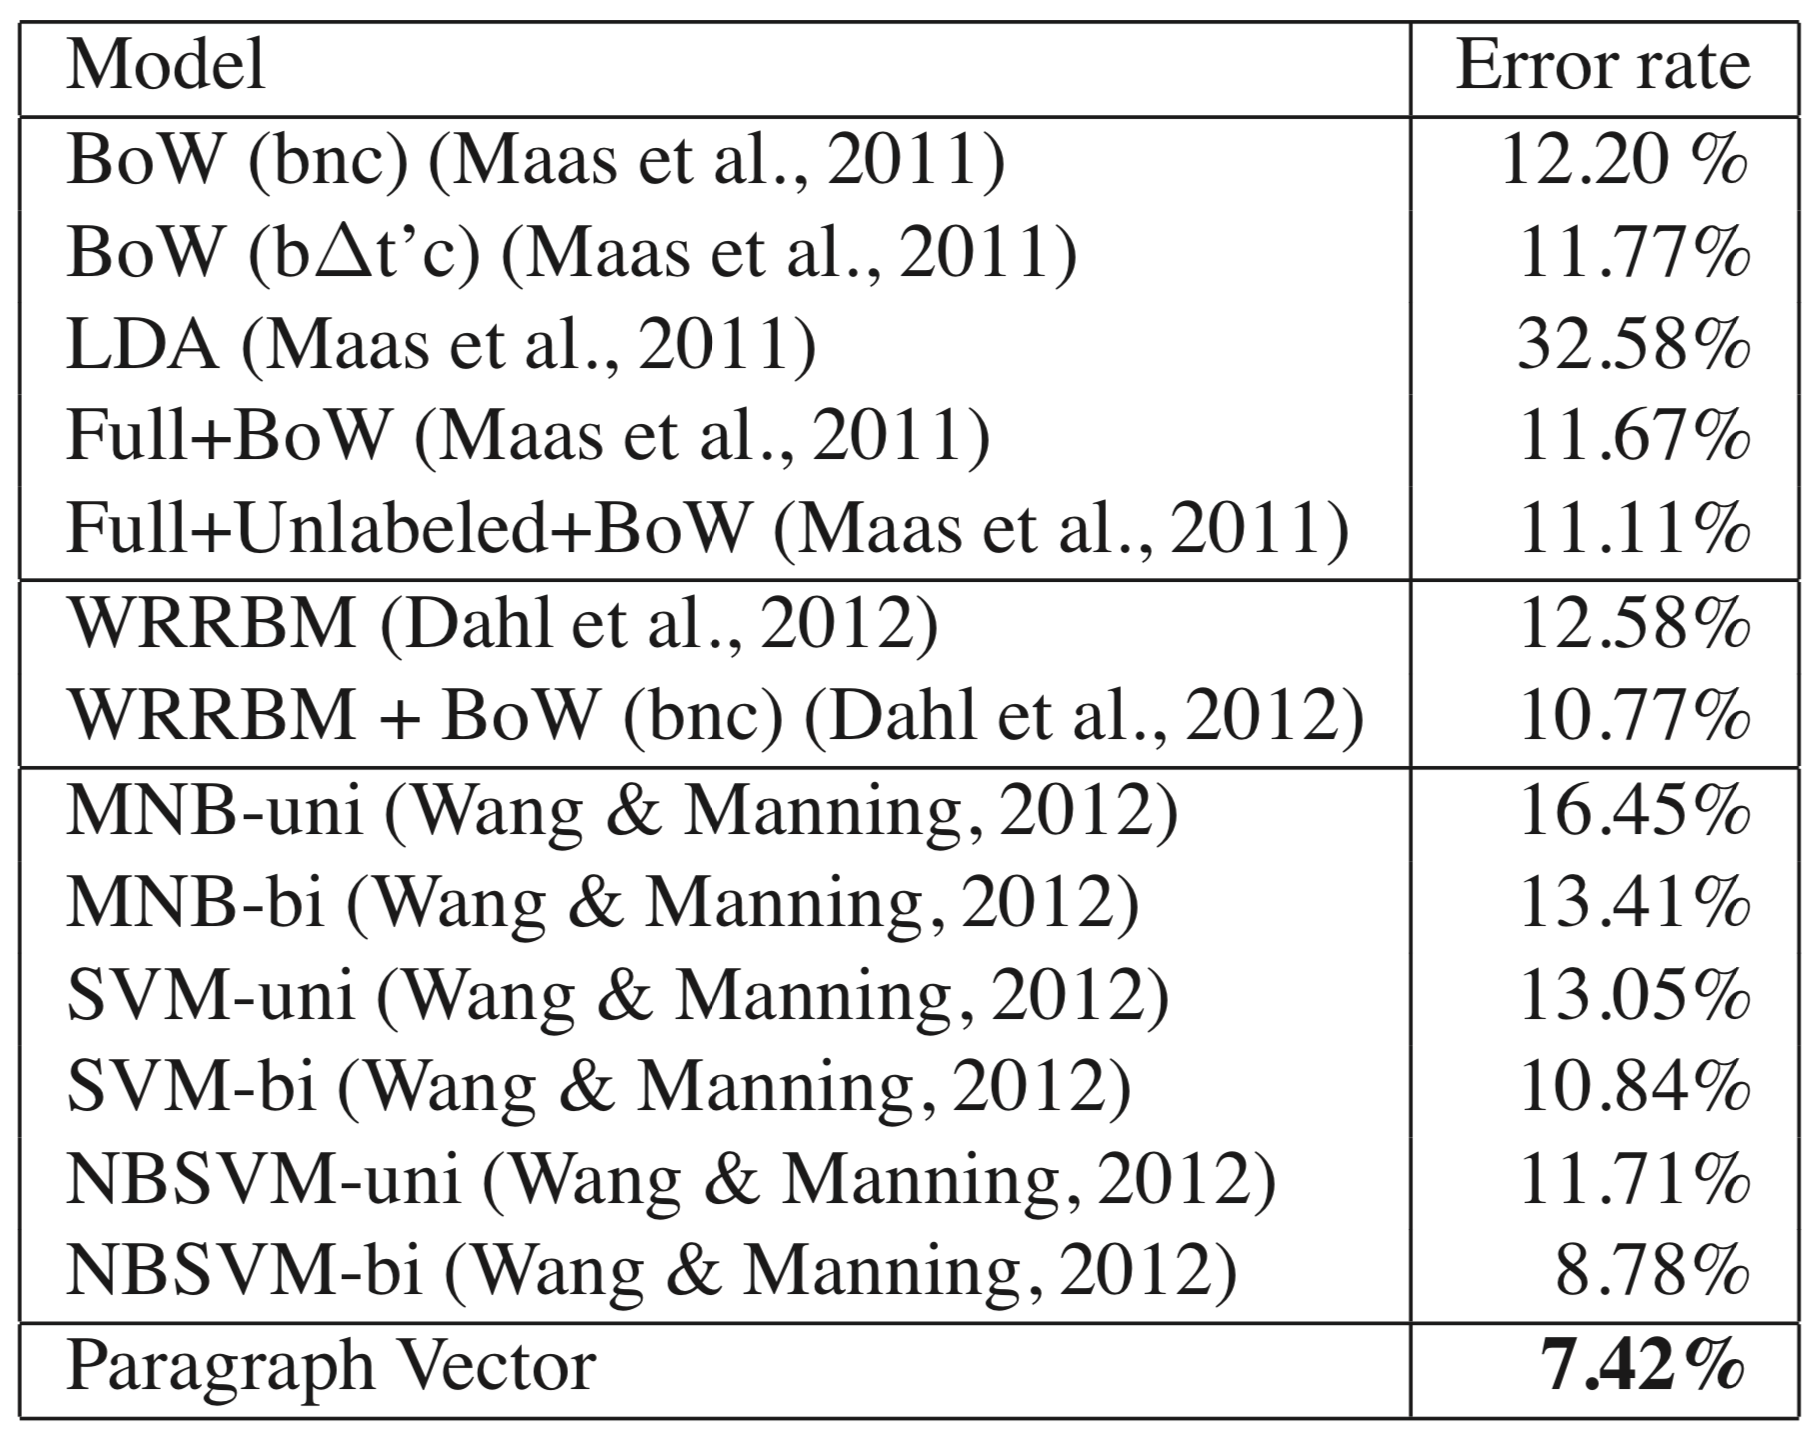
\includegraphics[width=.5\linewidth]{files/doc2vec-5.png}
  \caption{A variational autoencoder models the latent variable z from which the data x is generated.}
  \label{fig:vae}
\end{figure}

\begin{figure}
\centering
  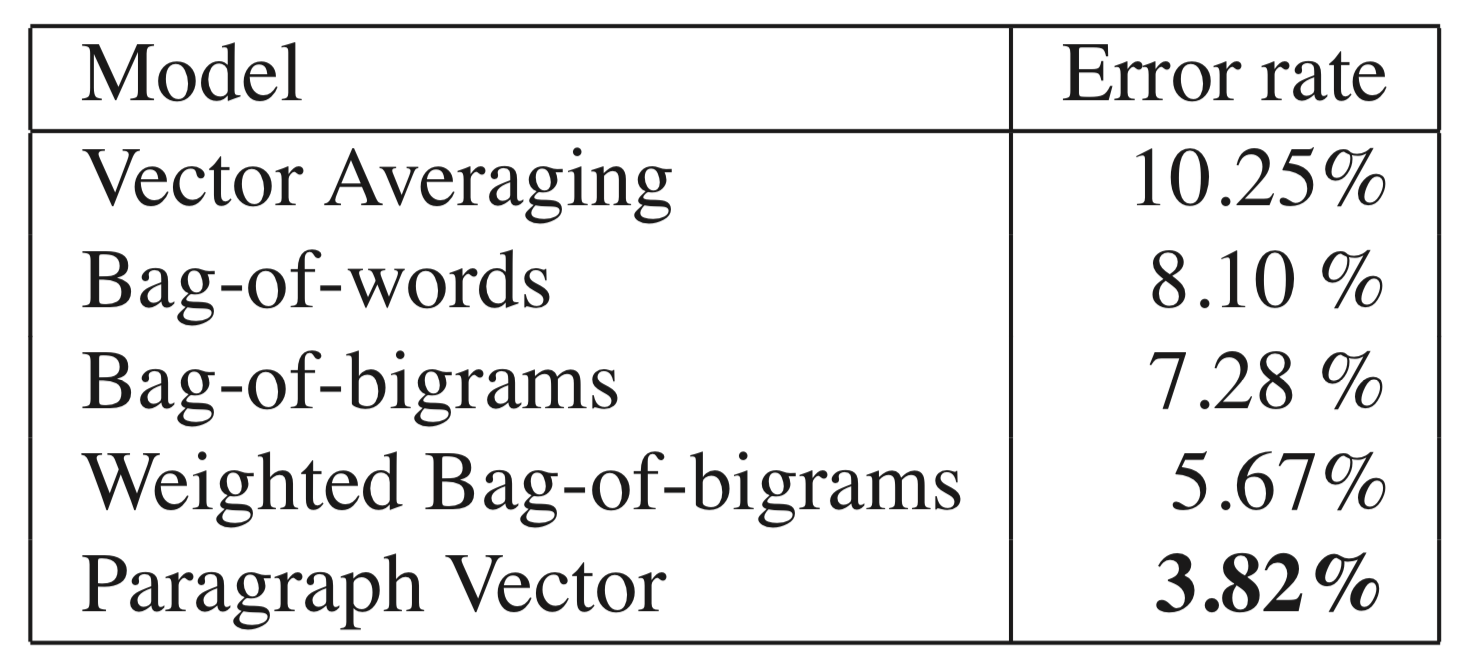
\includegraphics[width=.5\linewidth]{files/doc2vec-6.png}
  \caption{A variational autoencoder models the latent variable z from which the data x is generated.}
  \label{fig:vae}
\end{figure}


\subsection{Summary of Skip-thought Vectors}
% TODO same as previous subsection

Skip thoughts citation \cite{DBLP:journals/corr/KirosZSZTUF15}

\begin{figure}
\centering
  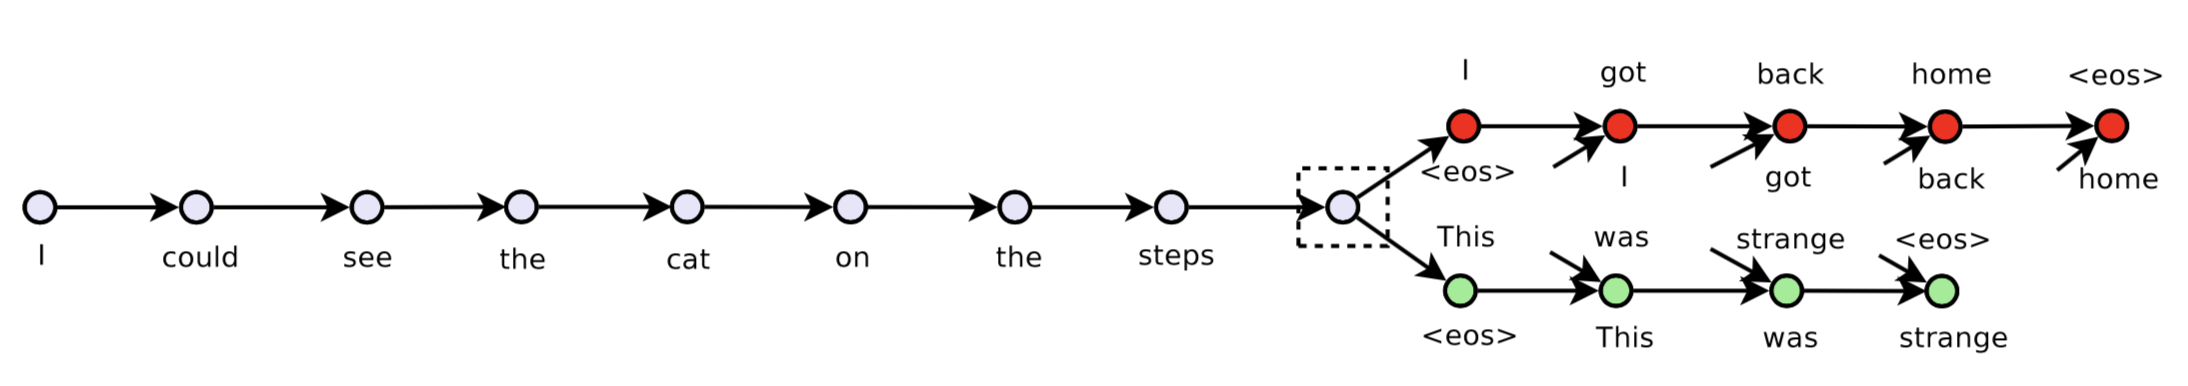
\includegraphics[width=.5\linewidth]{files/skipthoughts-1.png}
  \caption{A variational autoencoder models the latent variable z from which the data x is generated.}
  \label{fig:vae}
\end{figure}

\begin{figure}
\centering
  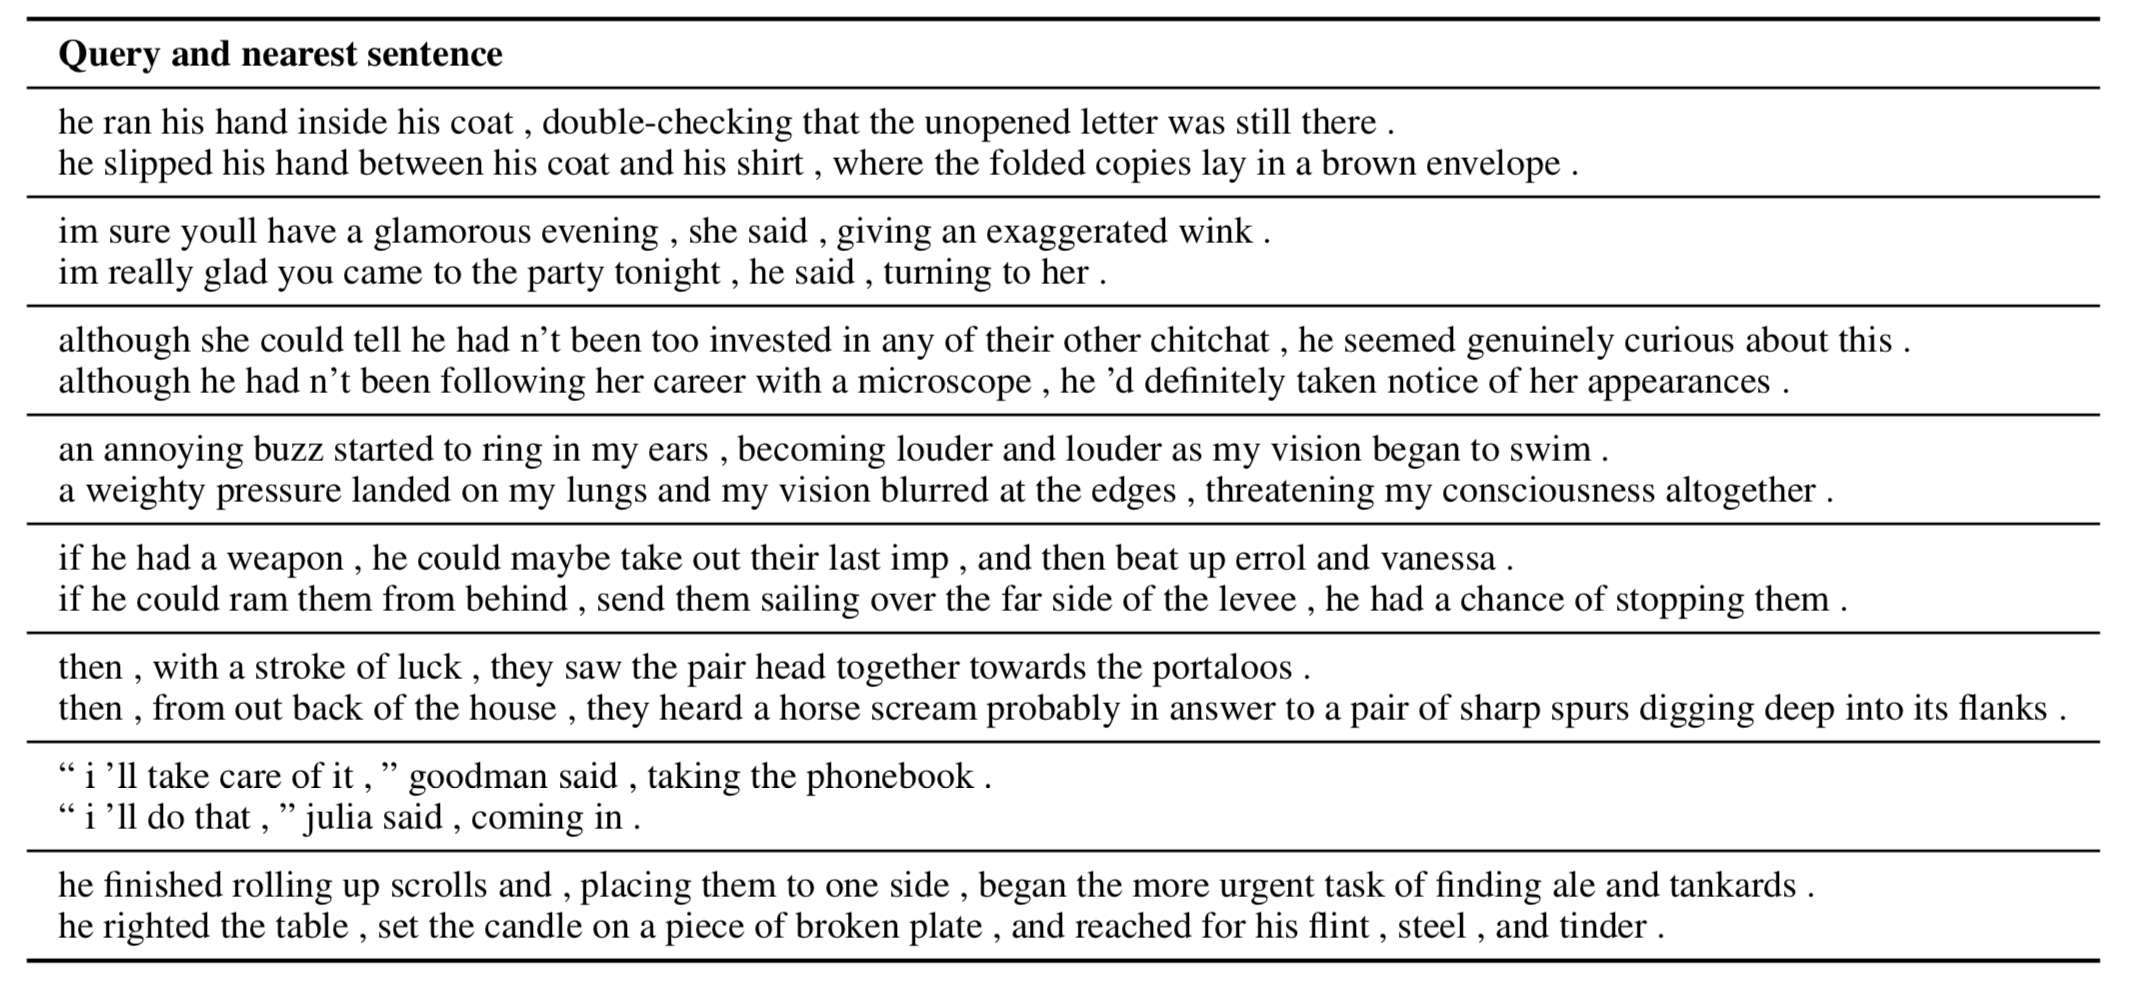
\includegraphics[width=.5\linewidth]{files/skipthoughts-2.png}
  \caption{A variational autoencoder models the latent variable z from which the data x is generated.}
  \label{fig:vae}
\end{figure}

\begin{figure}
\centering
  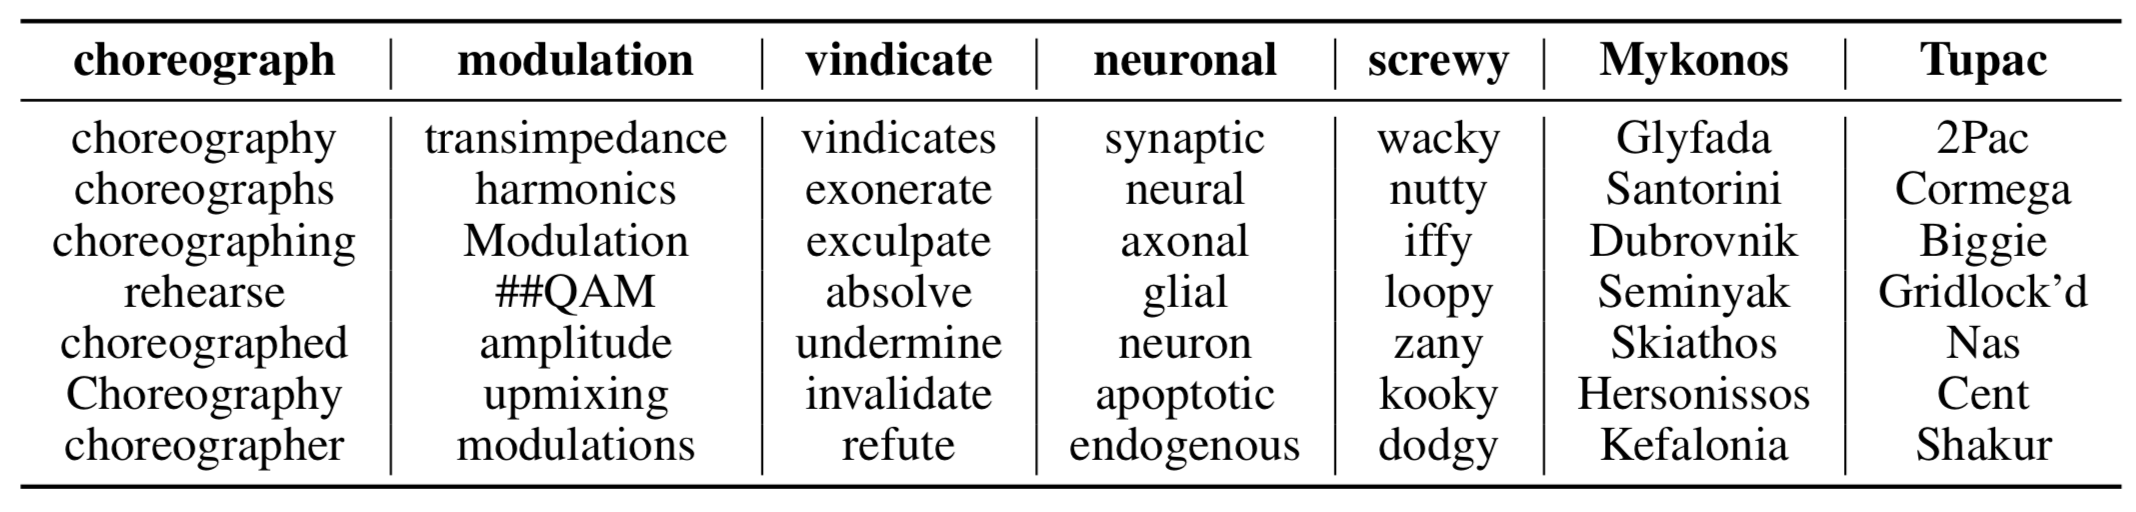
\includegraphics[width=.5\linewidth]{files/skipthoughts-3.png}
  \caption{A variational autoencoder models the latent variable z from which the data x is generated.}
  \label{fig:vae}
\end{figure}

\begin{figure}
\centering
  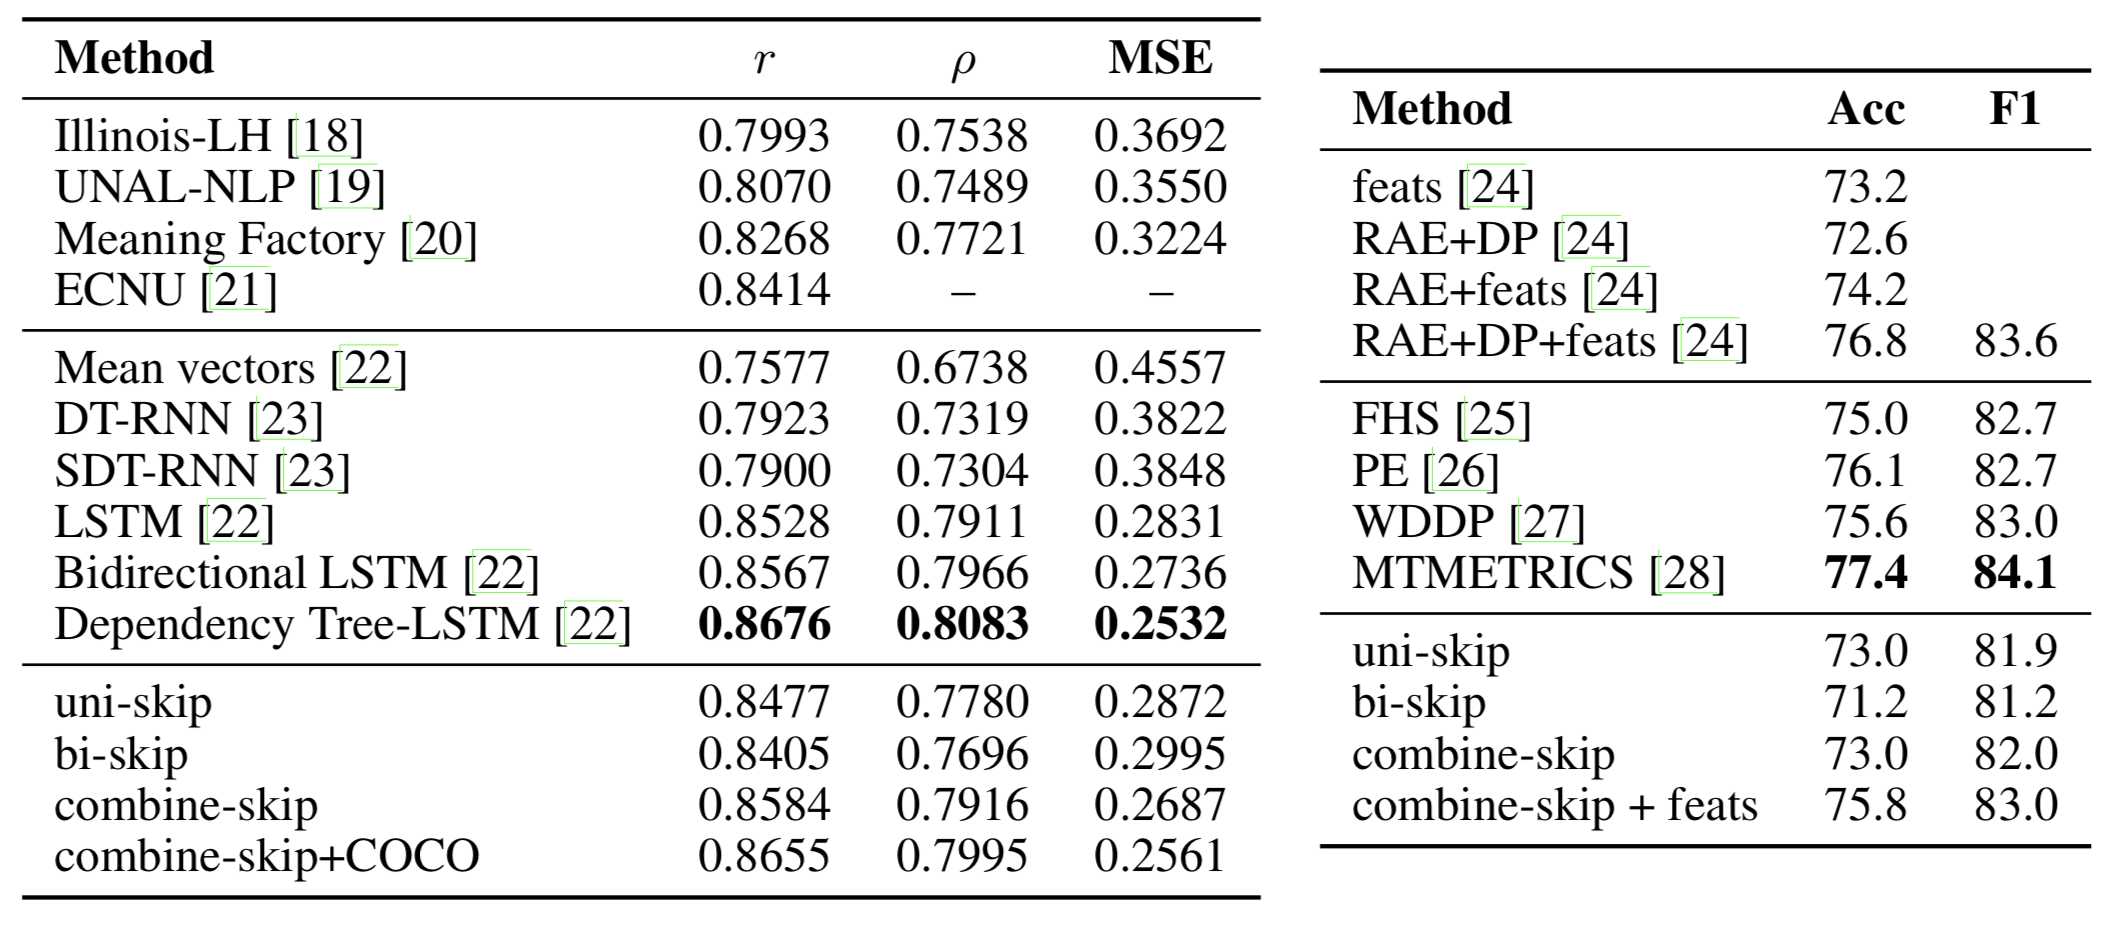
\includegraphics[width=.5\linewidth]{files/skipthoughts-4.png}
  \caption{A variational autoencoder models the latent variable z from which the data x is generated.}
  \label{fig:vae}
\end{figure}

\begin{figure}
\centering
  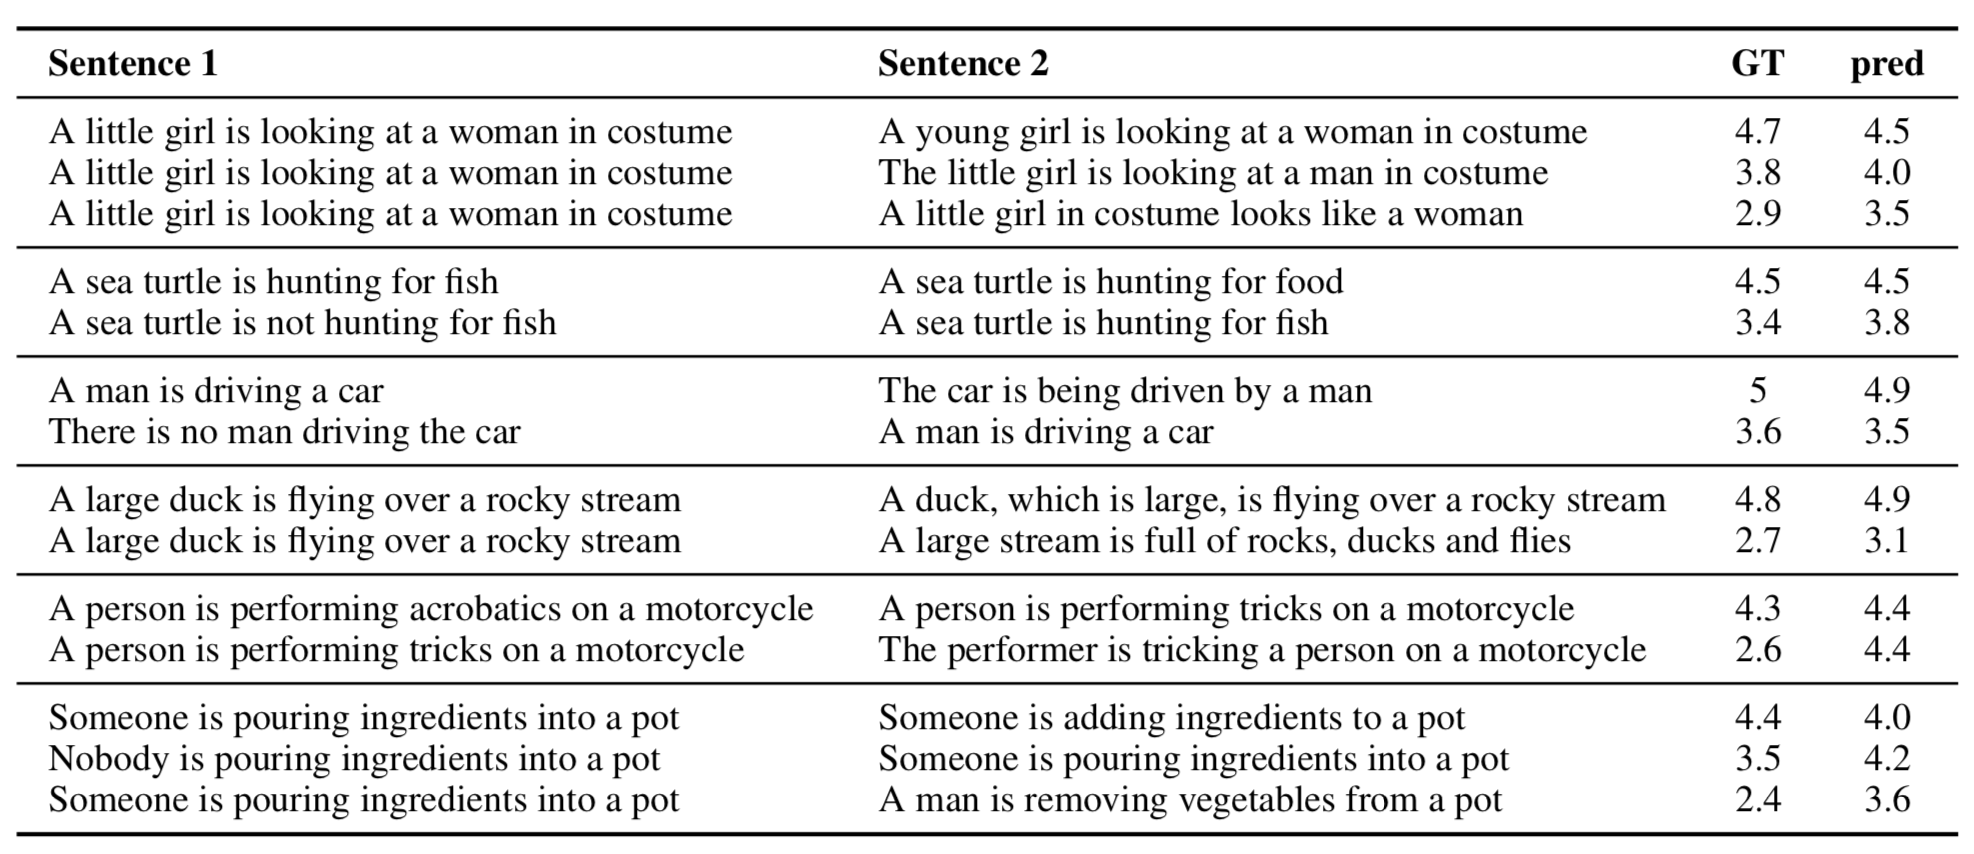
\includegraphics[width=.5\linewidth]{files/skipthoughts-5.png}
  \caption{A variational autoencoder models the latent variable z from which the data x is generated.}
  \label{fig:vae}
\end{figure}

\begin{figure}
\centering
  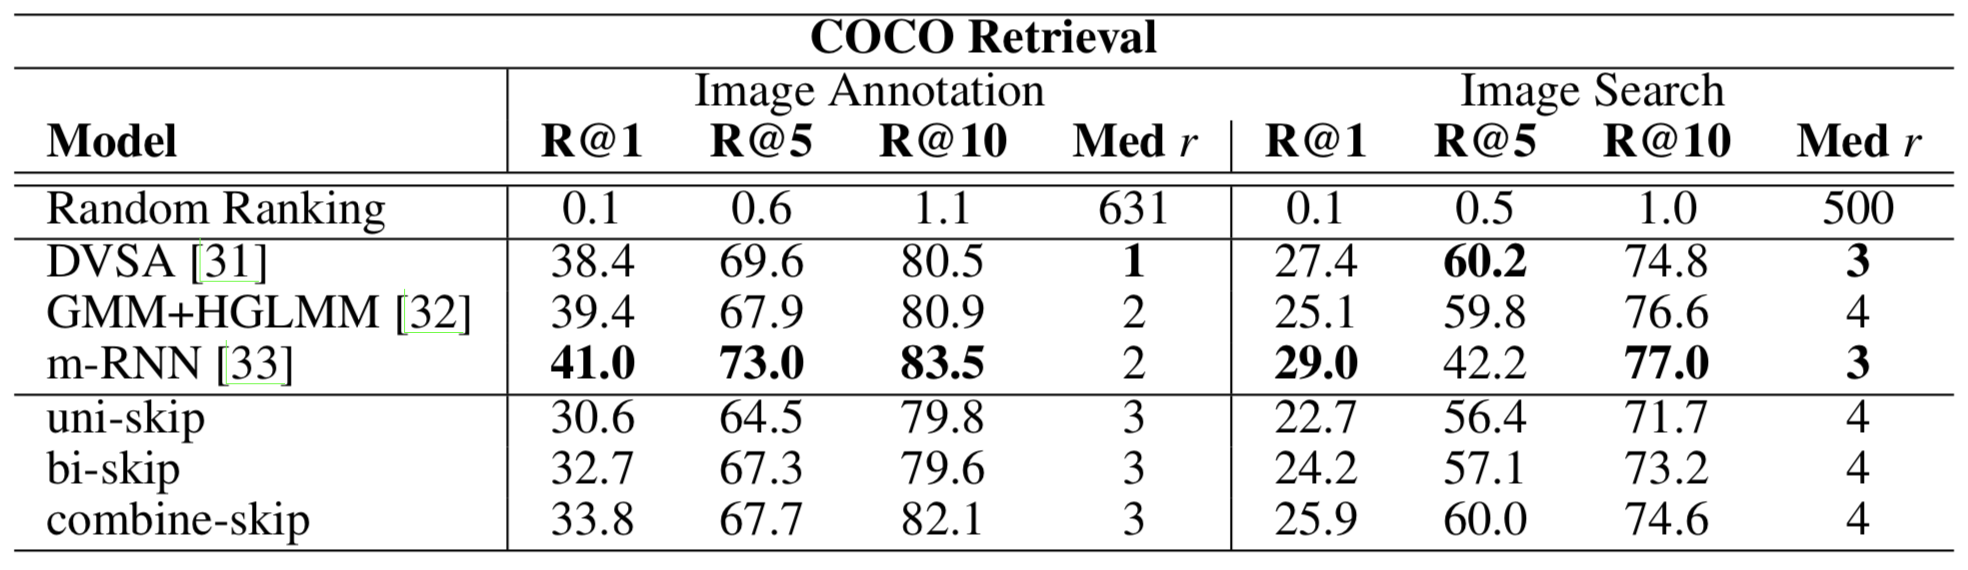
\includegraphics[width=.5\linewidth]{files/skipthoughts-6.png}
  \caption{A variational autoencoder models the latent variable z from which the data x is generated.}
  \label{fig:vae}
\end{figure}

\begin{figure}
\centering
  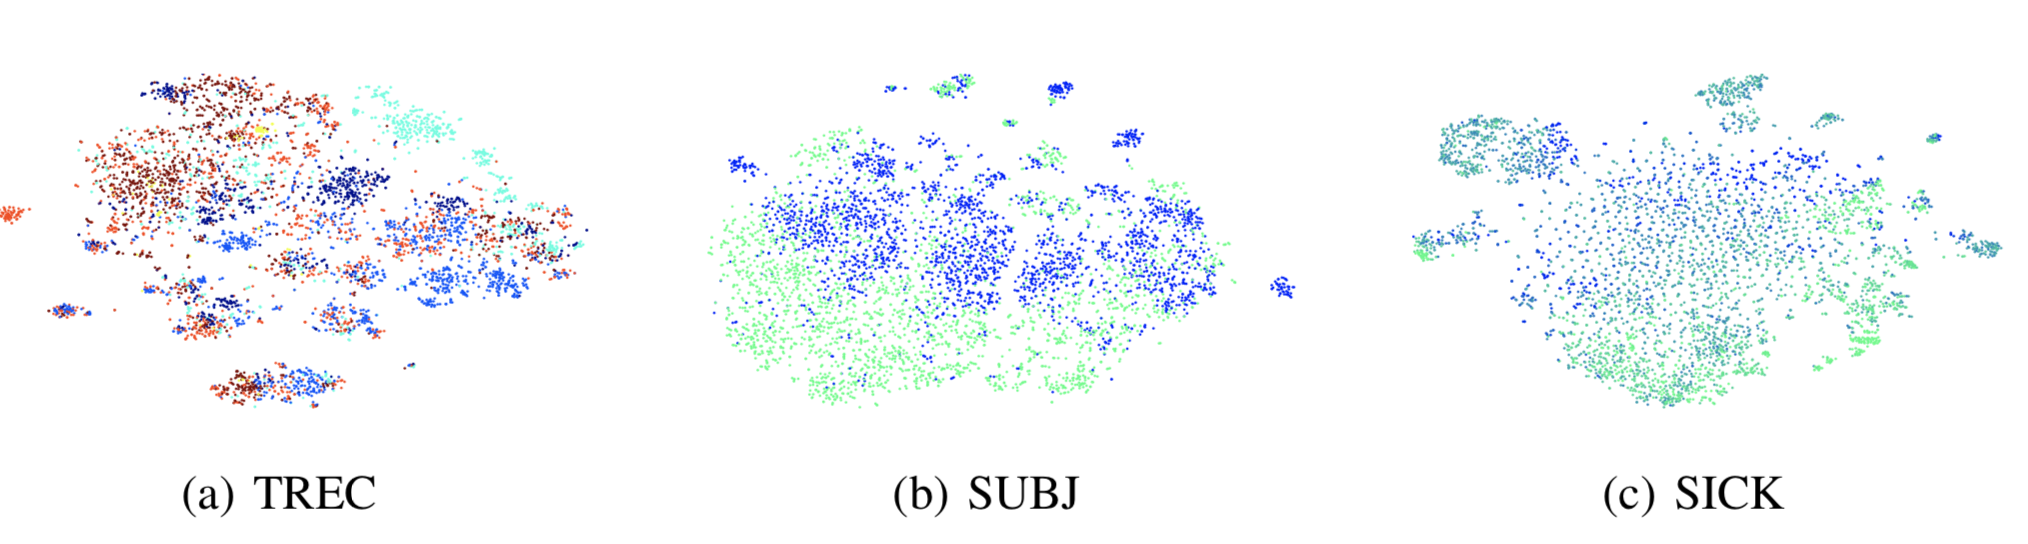
\includegraphics[width=.5\linewidth]{files/skipthoughts-7.png}
  \caption{A variational autoencoder models the latent variable z from which the data x is generated.}
  \label{fig:vae}
\end{figure}

\begin{figure}
\centering
  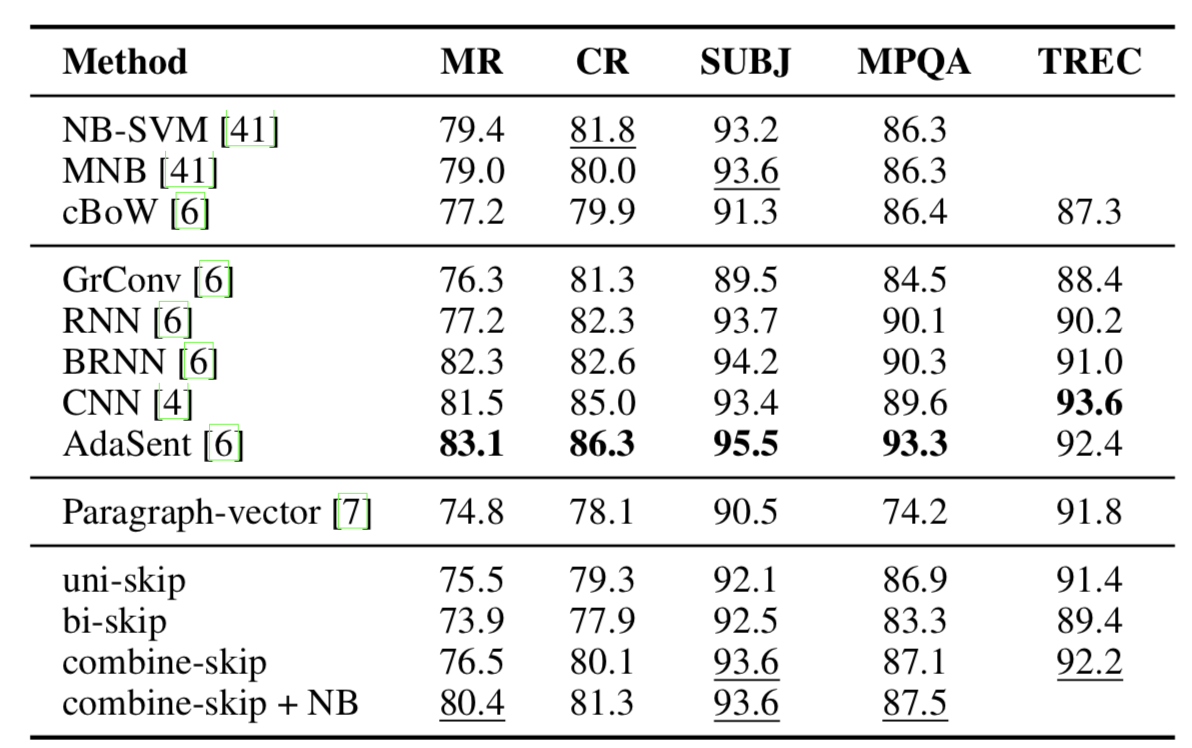
\includegraphics[width=.5\linewidth]{files/skipthoughts-8.png}
  \caption{A variational autoencoder models the latent variable z from which the data x is generated.}
  \label{fig:vae}
\end{figure}

\subsection{Summary of Distributed Representations of Sentences and Documents}
% TODO same as previous subsection

This is the citation for quick thoughts \cite{logeswaran2018an}.

\begin{figure}
\centering
  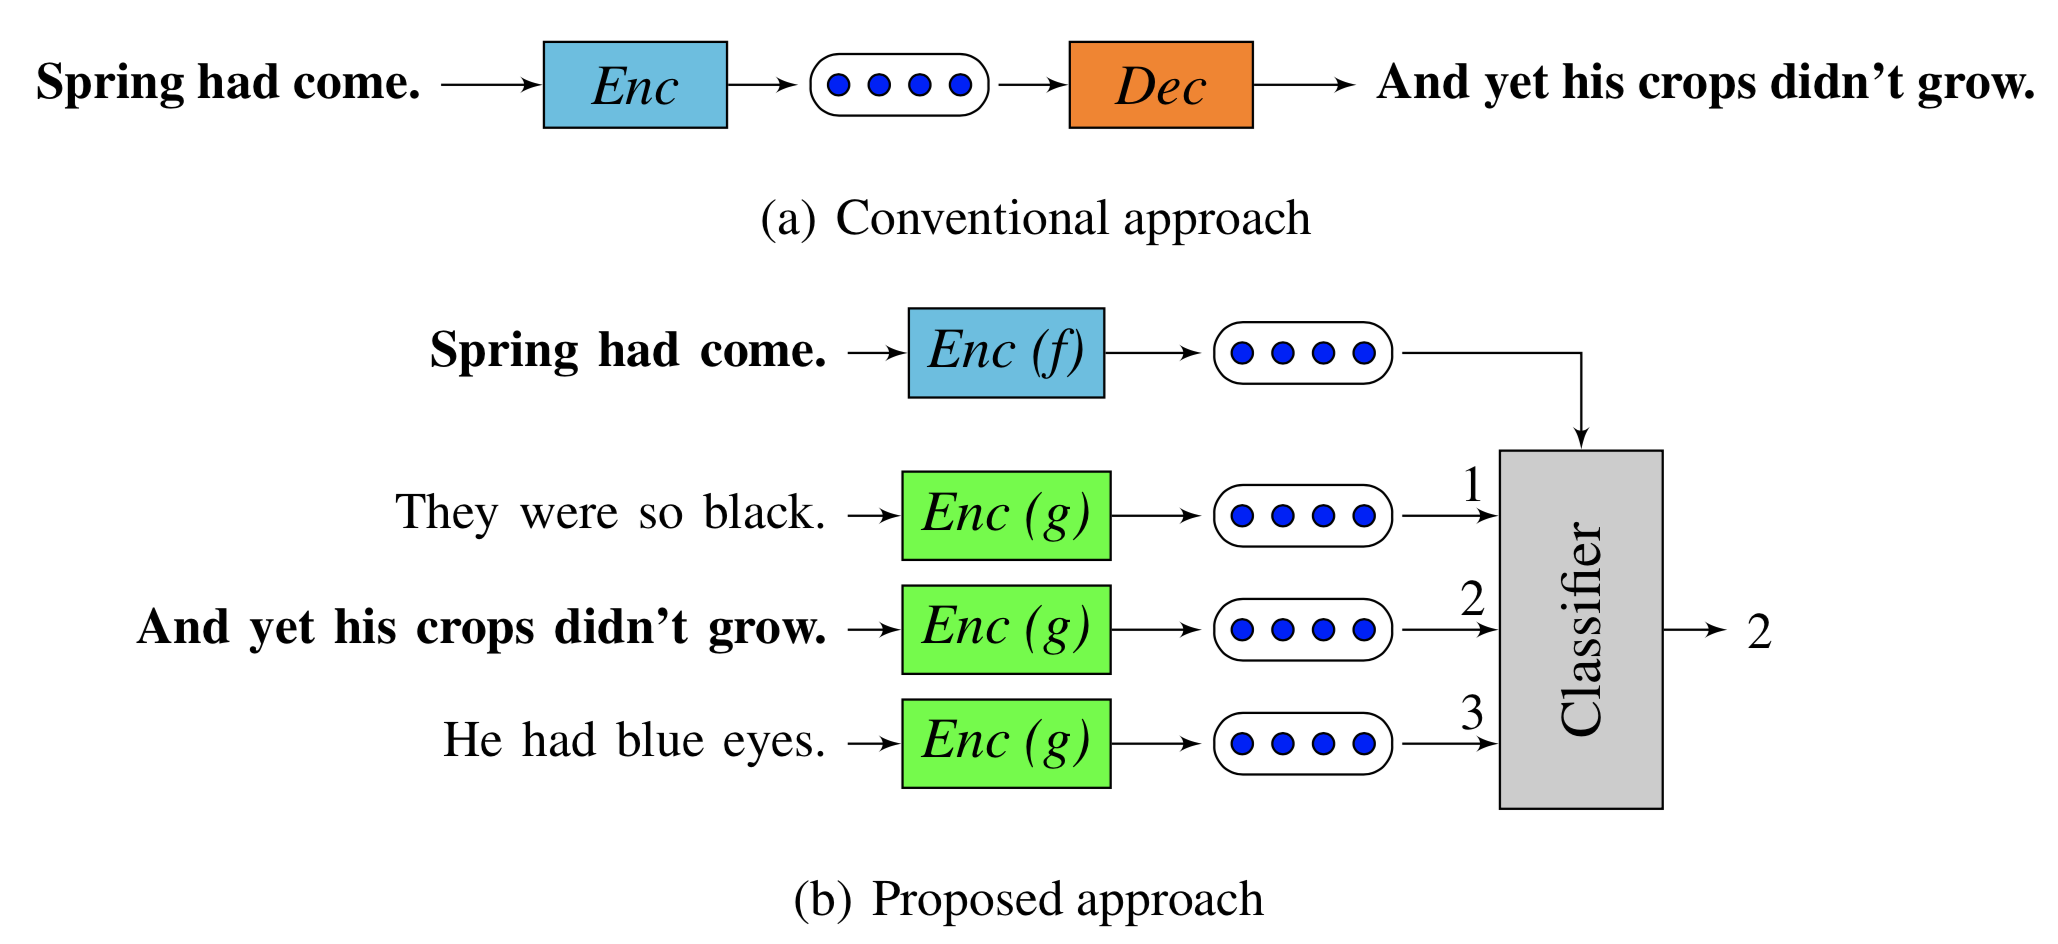
\includegraphics[width=.5\linewidth]{files/quickthoughts-1.png}
  \caption{Cap.}
  \label{fig:vae}
\end{figure}

\begin{figure}
\centering
  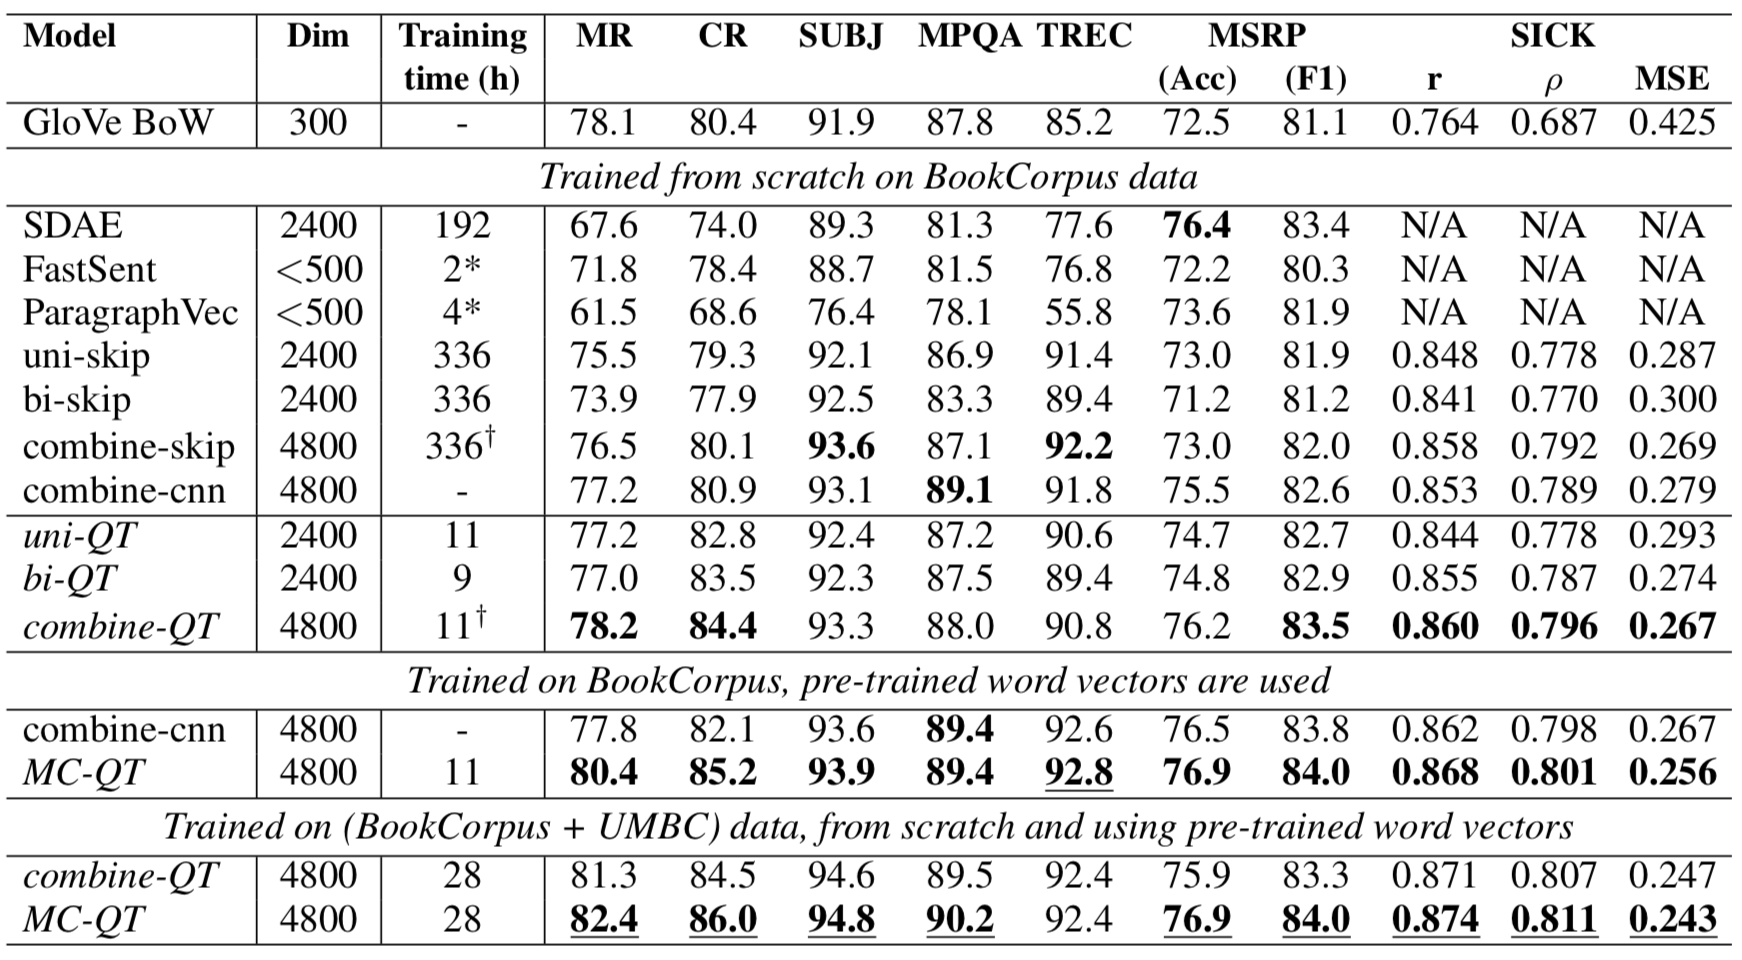
\includegraphics[width=.5\linewidth]{files/quickthoughts-2.png}
  \caption{Cap.}
  \label{fig:vae}
\end{figure}

\begin{figure}
\centering
  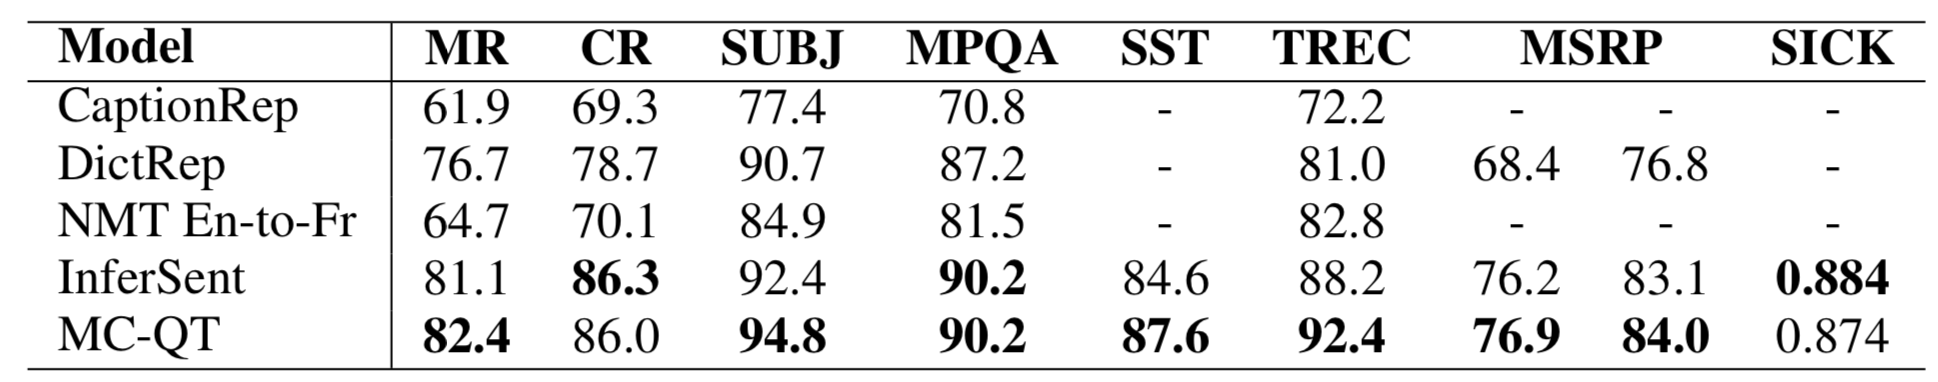
\includegraphics[width=.5\linewidth]{files/quickthoughts-3.png}
  \caption{Cap.}
  \label{fig:vae}
\end{figure}

\begin{figure}
\centering
  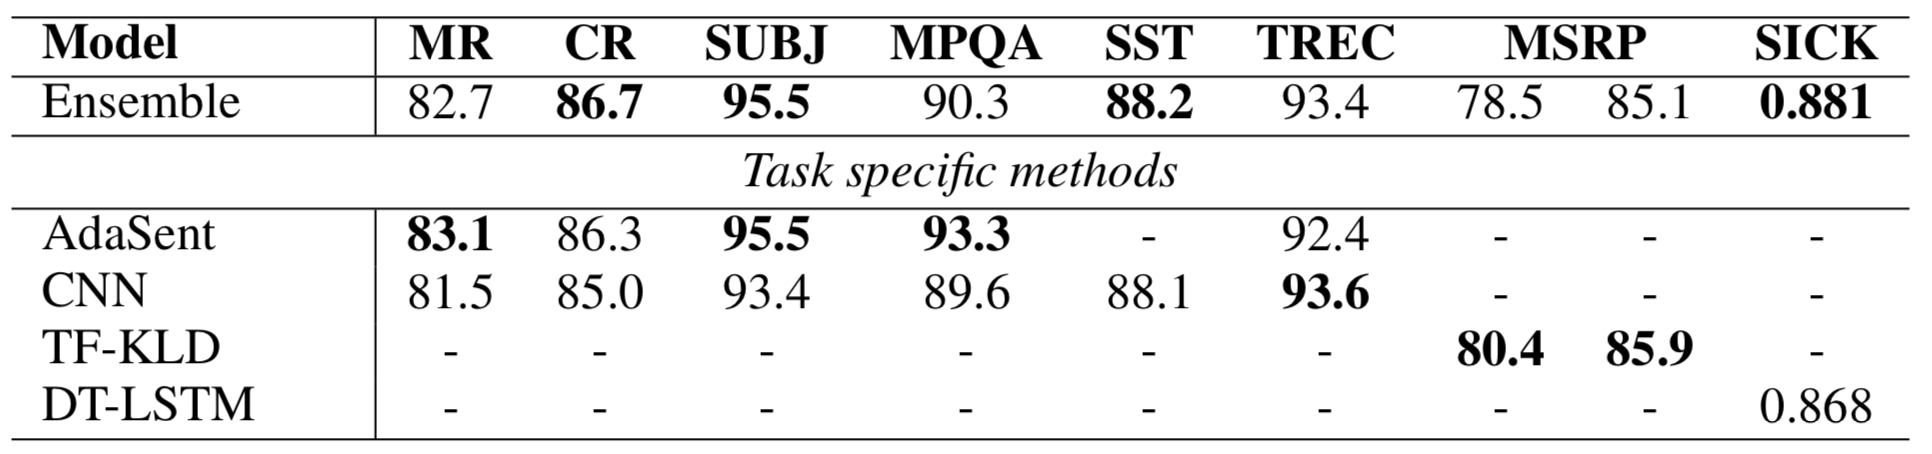
\includegraphics[width=.5\linewidth]{files/quickthoughts-4.png}
  \caption{Cap.}
  \label{fig:vae}
\end{figure}

\begin{figure}
\centering
  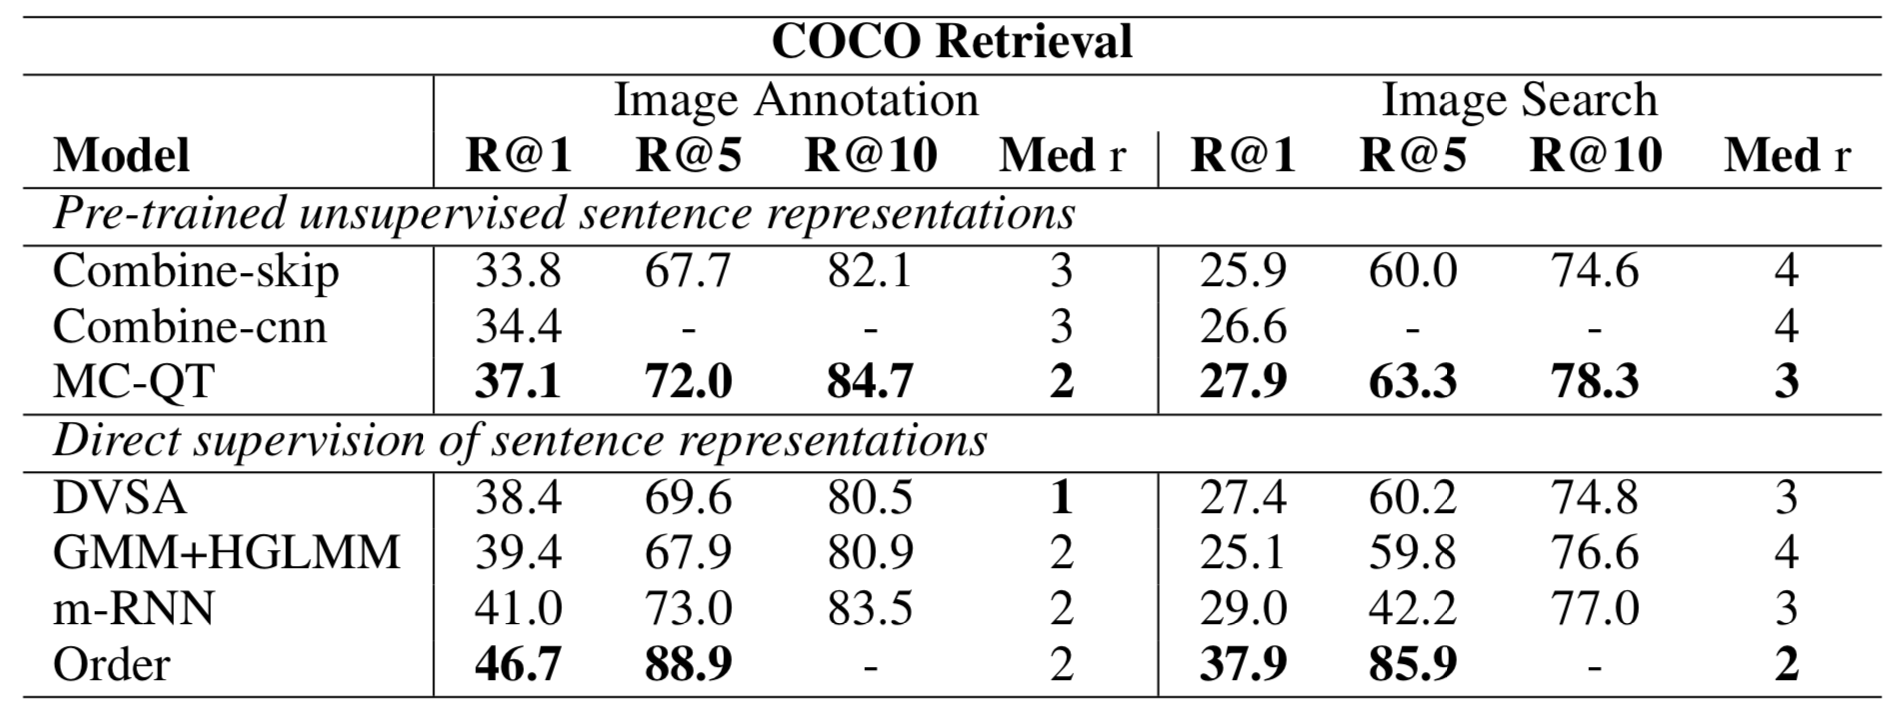
\includegraphics[width=.5\linewidth]{files/quickthoughts-5.png}
  \caption{Cap.}
  \label{fig:vae}
\end{figure}

\begin{figure}
\centering
  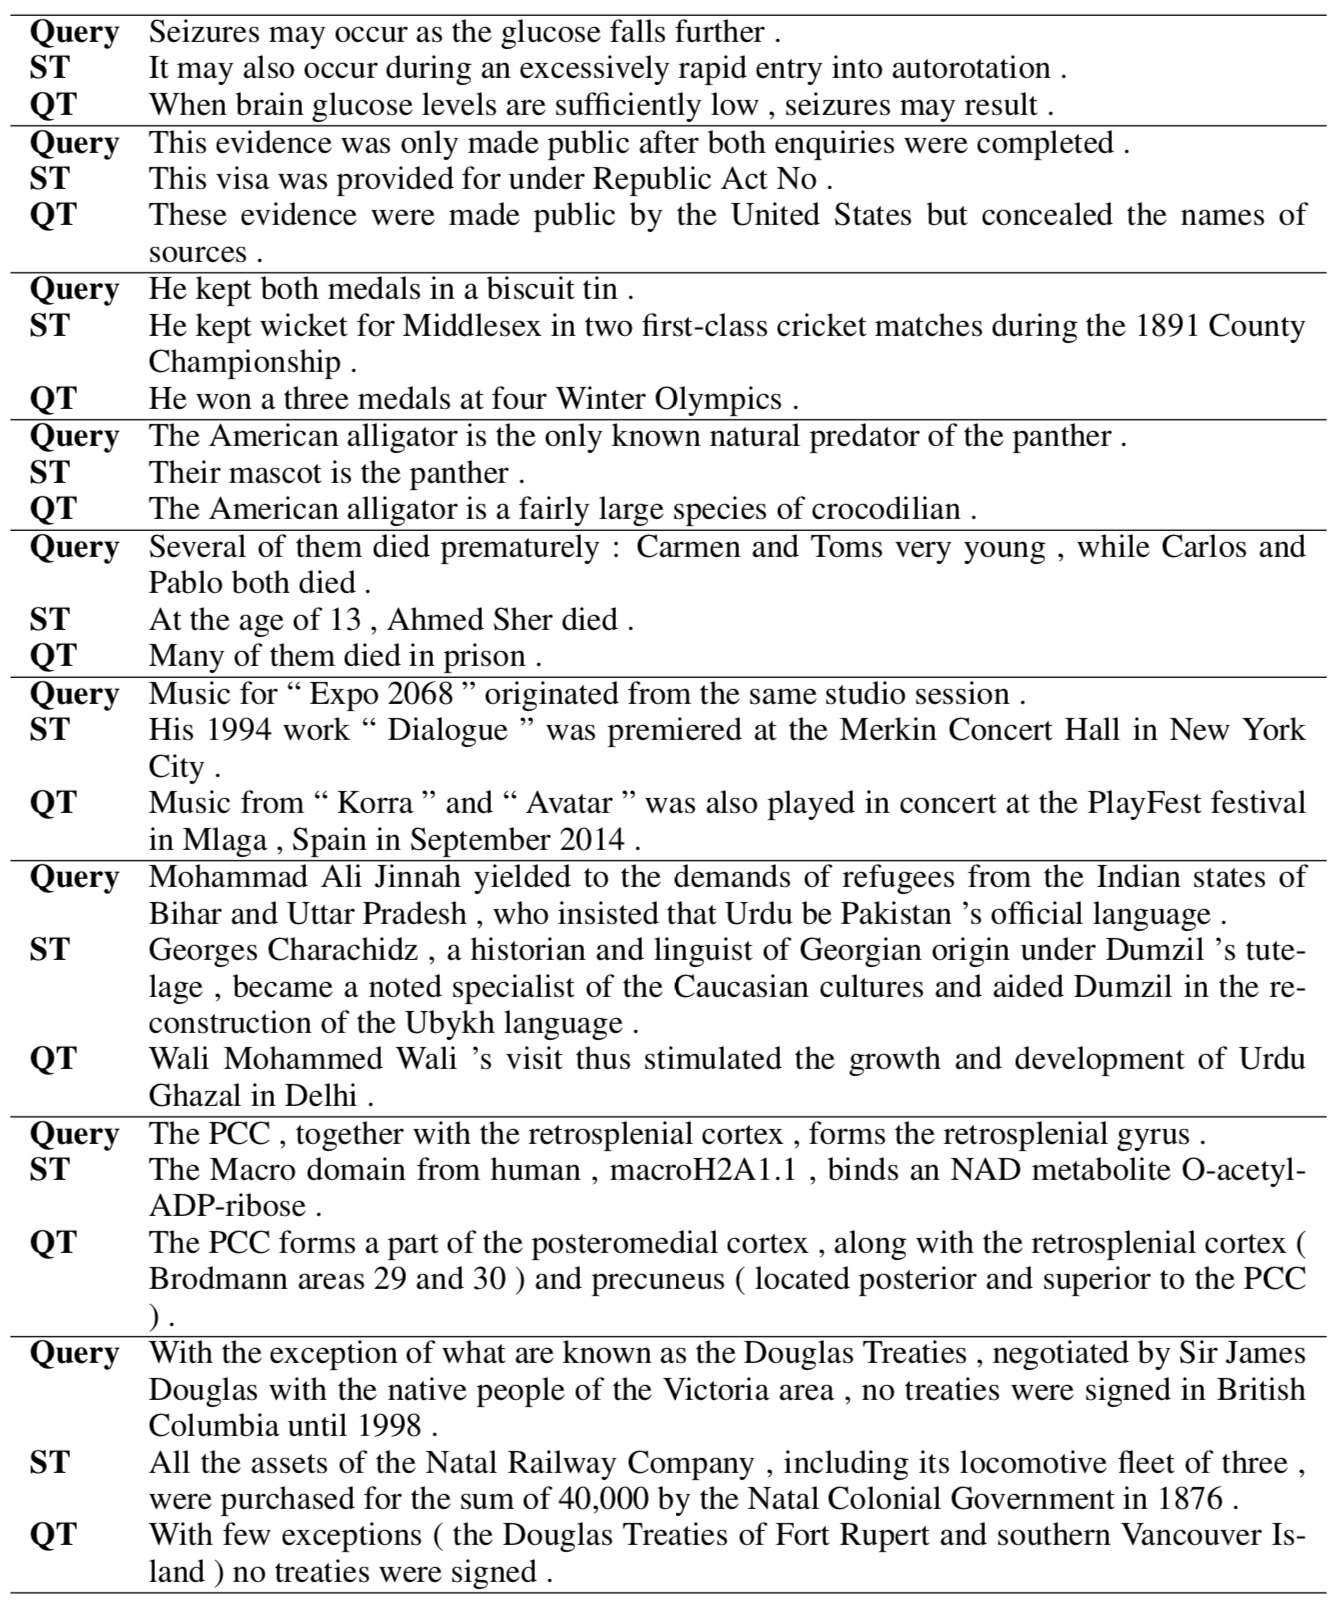
\includegraphics[width=.5\linewidth]{files/quickthoughts-6.png}
  \caption{Cap.}
  \label{fig:vae}
\end{figure}

\subsection{Summary of Universal Sentence Encoder}
% TODO same as previous subsection

Universal sentence encoder citation \cite{use}.

\begin{figure}
\centering
  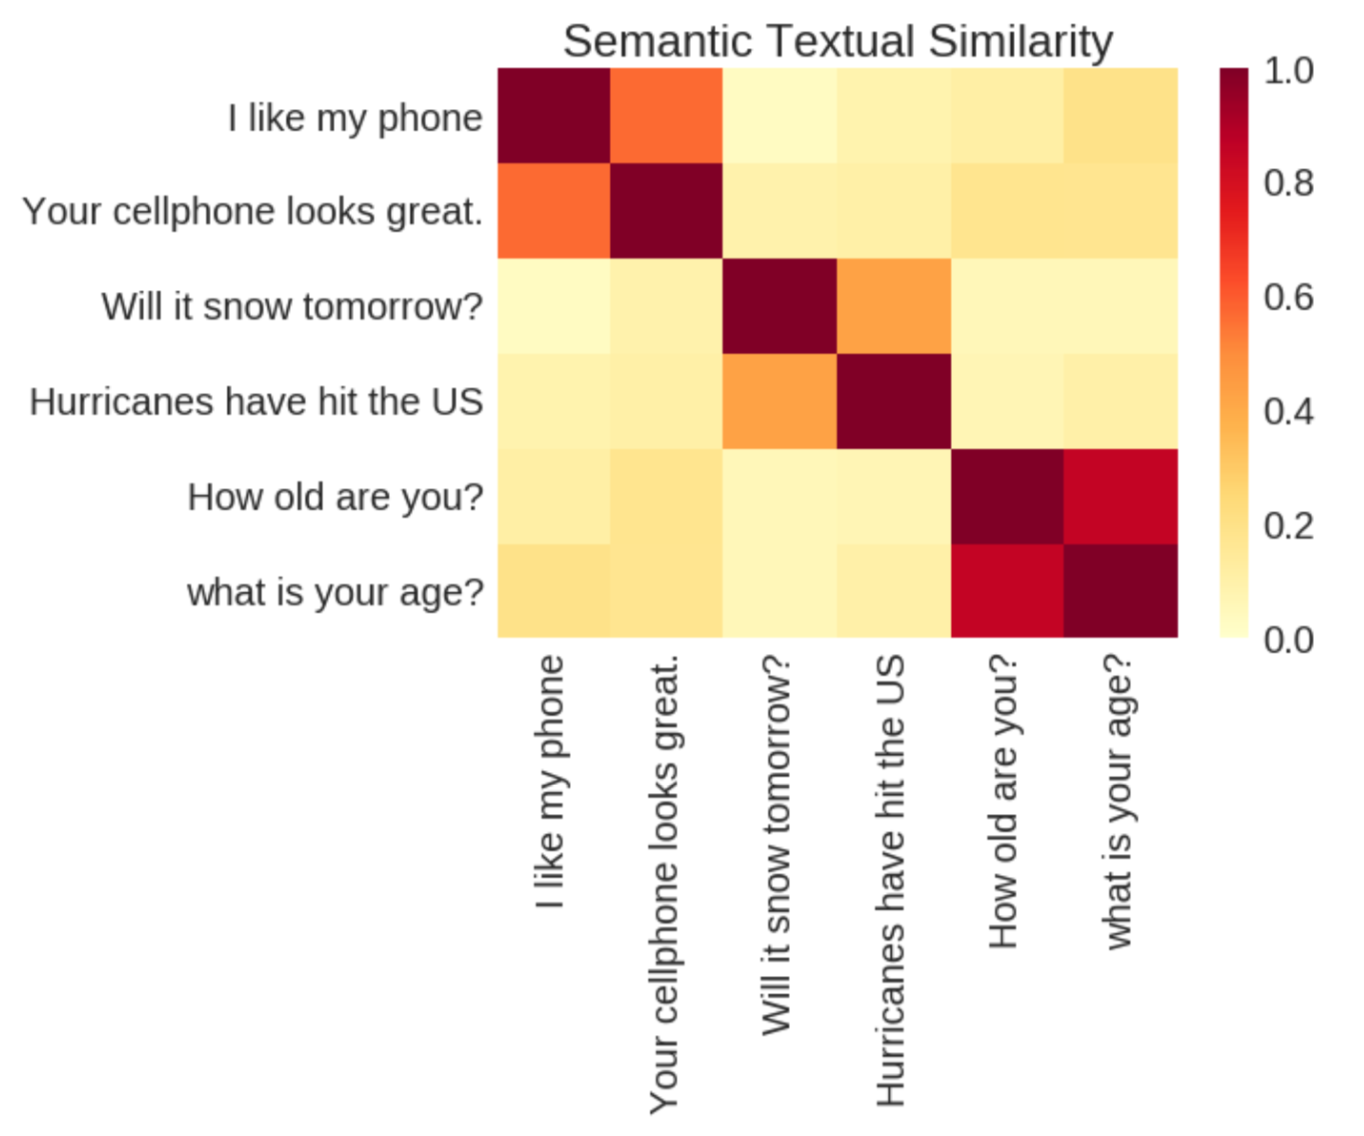
\includegraphics[width=.5\linewidth]{files/use-1.png}
  \caption{Cap.}
  \label{fig:vae}
\end{figure}

\begin{figure}
\centering
  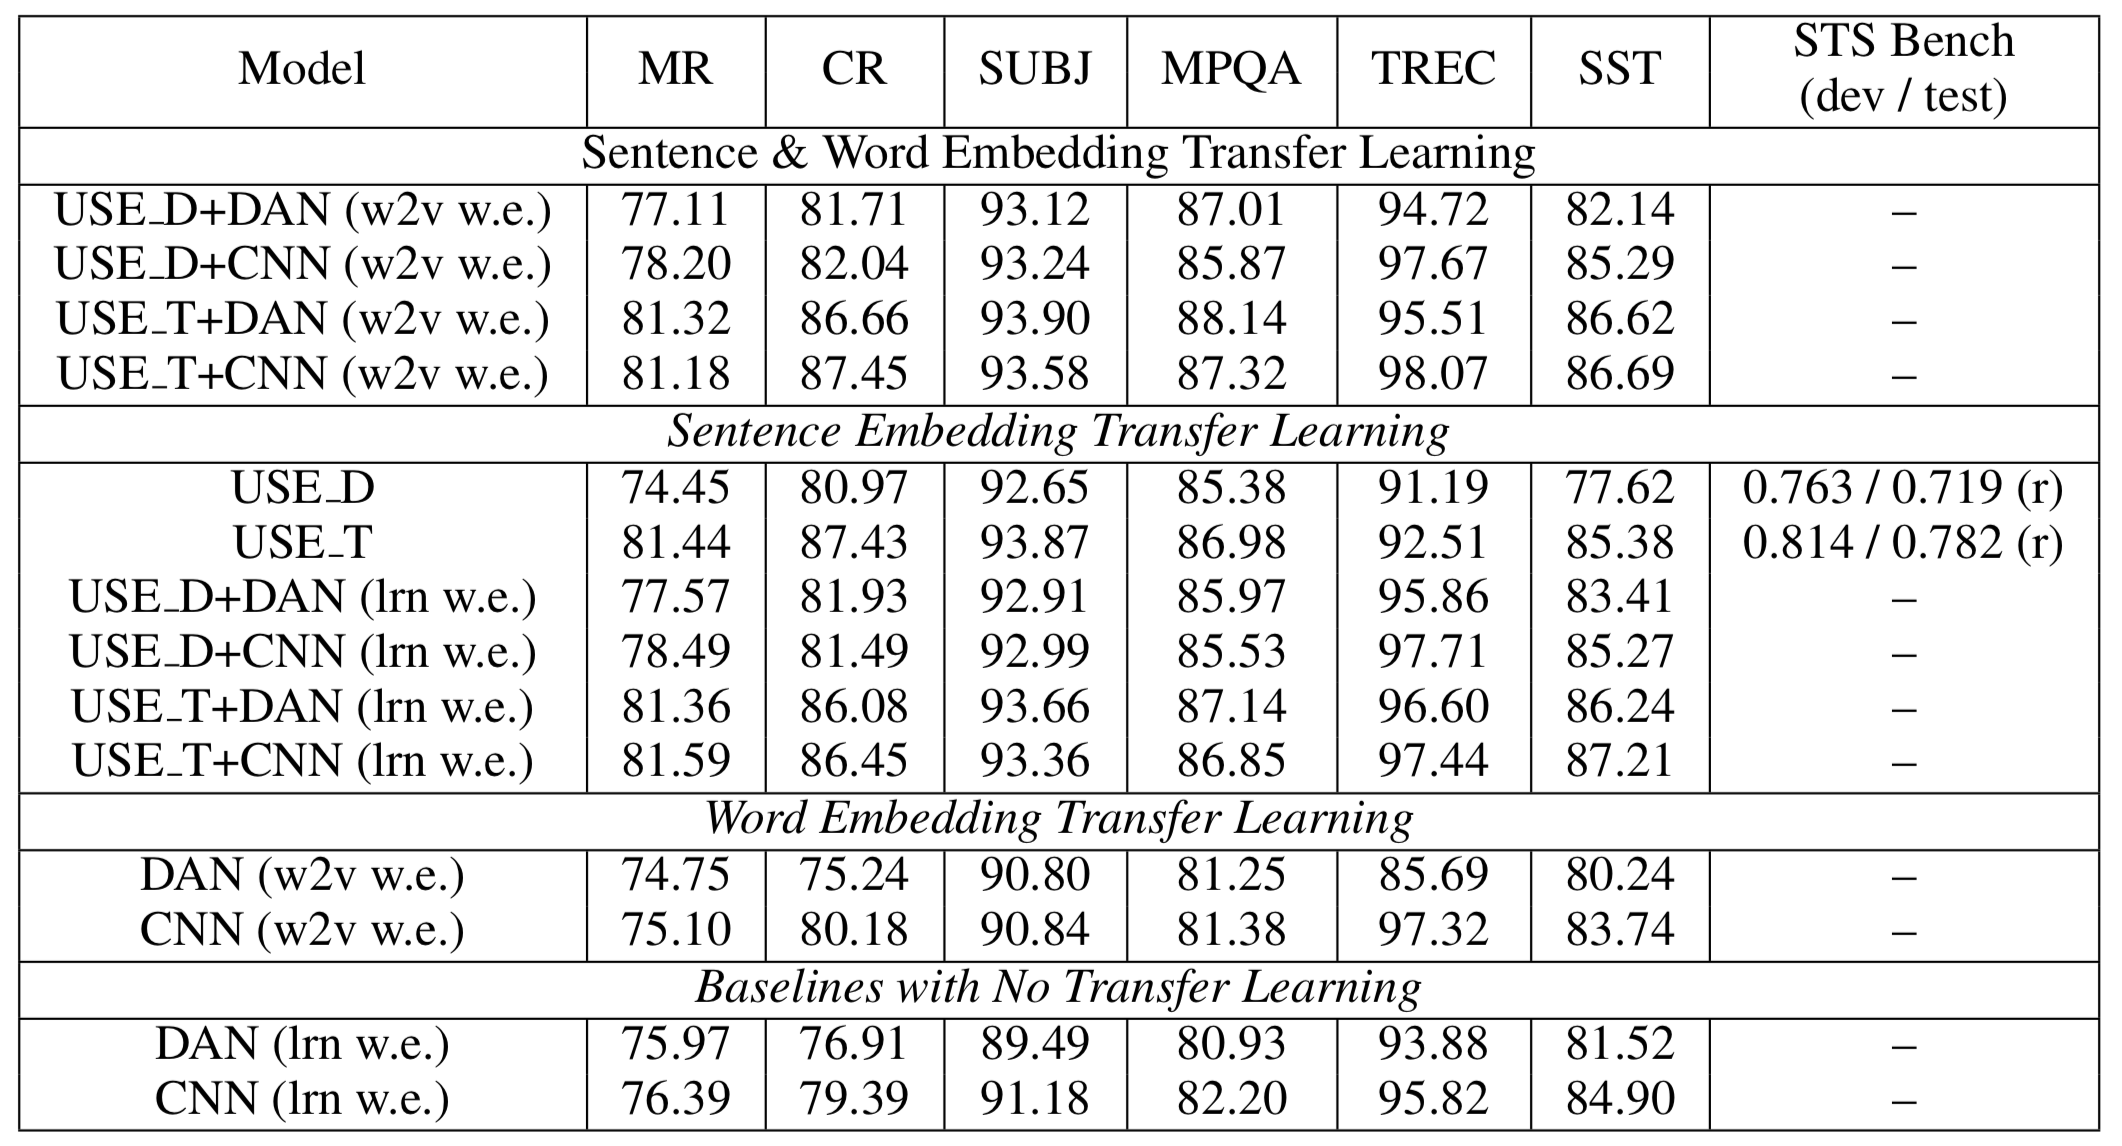
\includegraphics[width=.5\linewidth]{files/use-2.png}
  \caption{Cap.}
  \label{fig:vae}
\end{figure}

\begin{figure}
\centering
  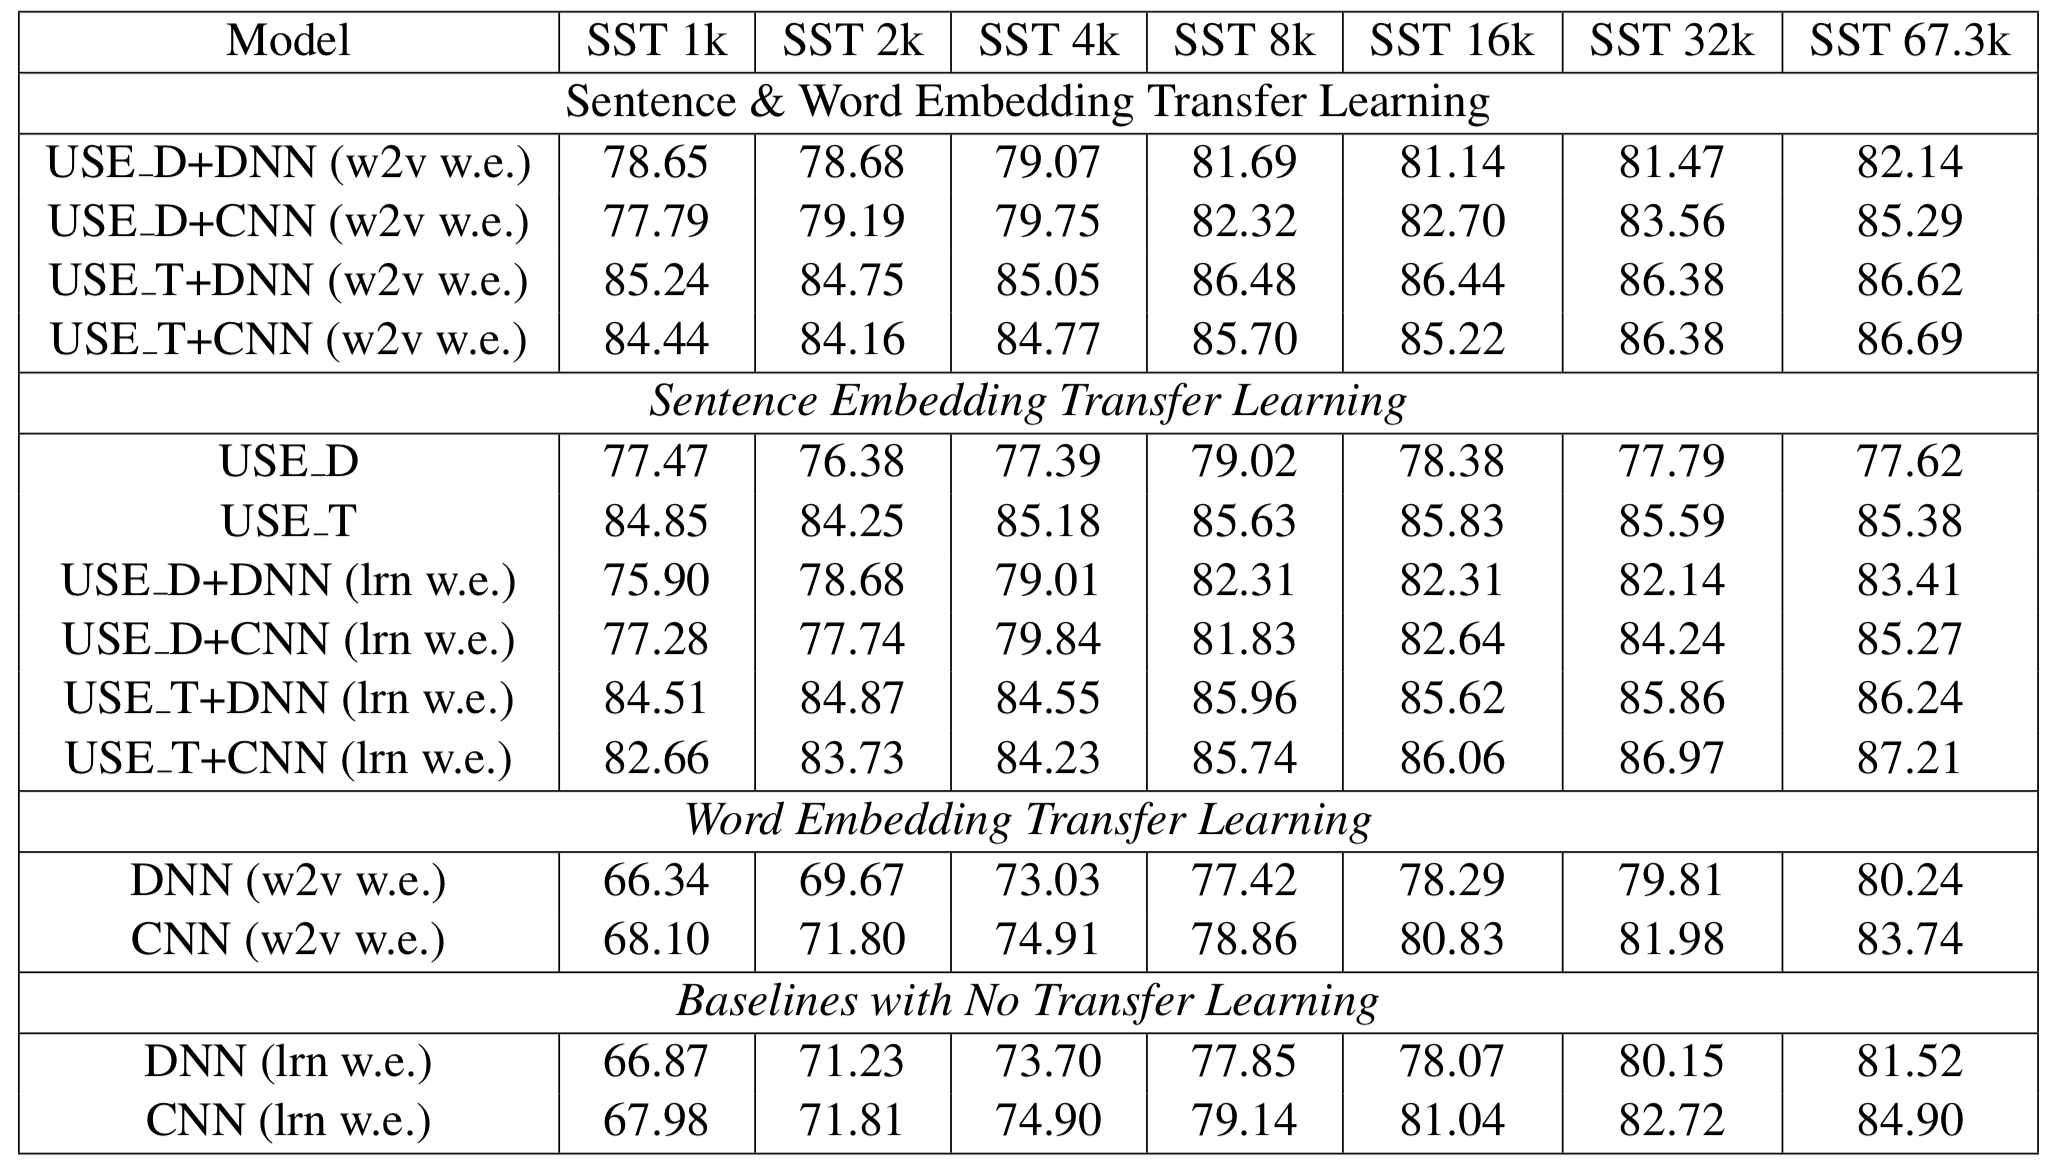
\includegraphics[width=.5\linewidth]{files/use-3.png}
  \caption{Cap.}
  \label{fig:vae}
\end{figure}

\section{\label{sec:level5} Comparison of Papers}
% TODO Give a short overview/comparison of the methods discussed in the papers

\section{\label{sec:level6} Summary}
% Conclude the presentation/make any final brief statements. This is not a summary like the introduction. 
